% interactcadsample.tex
% v1.03 - April 2017

\documentclass[]{interact}

\usepackage{epstopdf}% To incorporate .eps illustrations using PDFLaTeX, etc.
\usepackage{subfigure}% Support for small, `sub' figures and tables
%\usepackage[nolists,tablesfirst]{endfloat}% To `separate' figures and tables from text if required

\usepackage{natbib}% Citation support using natbib.sty
\bibpunct[, ]{(}{)}{;}{a}{}{,}% Citation support using natbib.sty
\renewcommand\bibfont{\fontsize{10}{12}\selectfont}% Bibliography support using natbib.sty

\theoremstyle{plain}% Theorem-like structures provided by amsthm.sty
\newtheorem{theorem}{Theorem}[section]
\newtheorem{lemma}[theorem]{Lemma}
\newtheorem{corollary}[theorem]{Corollary}
\newtheorem{proposition}[theorem]{Proposition}

\theoremstyle{definition}
\newtheorem{definition}[theorem]{Definition}
\newtheorem{example}[theorem]{Example}

\theoremstyle{remark}
\newtheorem{remark}{Remark}
\newtheorem{notation}{Notation}

% Pandoc syntax highlighting
\usepackage{color}
\usepackage{fancyvrb}
\newcommand{\VerbBar}{|}
\newcommand{\VERB}{\Verb[commandchars=\\\{\}]}
\DefineVerbatimEnvironment{Highlighting}{Verbatim}{commandchars=\\\{\}}
% Add ',fontsize=\small' for more characters per line
\usepackage{framed}
\definecolor{shadecolor}{RGB}{248,248,248}
\newenvironment{Shaded}{\begin{snugshade}}{\end{snugshade}}
\newcommand{\AlertTok}[1]{\textcolor[rgb]{0.94,0.16,0.16}{#1}}
\newcommand{\AnnotationTok}[1]{\textcolor[rgb]{0.56,0.35,0.01}{\textbf{\textit{#1}}}}
\newcommand{\AttributeTok}[1]{\textcolor[rgb]{0.77,0.63,0.00}{#1}}
\newcommand{\BaseNTok}[1]{\textcolor[rgb]{0.00,0.00,0.81}{#1}}
\newcommand{\BuiltInTok}[1]{#1}
\newcommand{\CharTok}[1]{\textcolor[rgb]{0.31,0.60,0.02}{#1}}
\newcommand{\CommentTok}[1]{\textcolor[rgb]{0.56,0.35,0.01}{\textit{#1}}}
\newcommand{\CommentVarTok}[1]{\textcolor[rgb]{0.56,0.35,0.01}{\textbf{\textit{#1}}}}
\newcommand{\ConstantTok}[1]{\textcolor[rgb]{0.00,0.00,0.00}{#1}}
\newcommand{\ControlFlowTok}[1]{\textcolor[rgb]{0.13,0.29,0.53}{\textbf{#1}}}
\newcommand{\DataTypeTok}[1]{\textcolor[rgb]{0.13,0.29,0.53}{#1}}
\newcommand{\DecValTok}[1]{\textcolor[rgb]{0.00,0.00,0.81}{#1}}
\newcommand{\DocumentationTok}[1]{\textcolor[rgb]{0.56,0.35,0.01}{\textbf{\textit{#1}}}}
\newcommand{\ErrorTok}[1]{\textcolor[rgb]{0.64,0.00,0.00}{\textbf{#1}}}
\newcommand{\ExtensionTok}[1]{#1}
\newcommand{\FloatTok}[1]{\textcolor[rgb]{0.00,0.00,0.81}{#1}}
\newcommand{\FunctionTok}[1]{\textcolor[rgb]{0.00,0.00,0.00}{#1}}
\newcommand{\ImportTok}[1]{#1}
\newcommand{\InformationTok}[1]{\textcolor[rgb]{0.56,0.35,0.01}{\textbf{\textit{#1}}}}
\newcommand{\KeywordTok}[1]{\textcolor[rgb]{0.13,0.29,0.53}{\textbf{#1}}}
\newcommand{\NormalTok}[1]{#1}
\newcommand{\OperatorTok}[1]{\textcolor[rgb]{0.81,0.36,0.00}{\textbf{#1}}}
\newcommand{\OtherTok}[1]{\textcolor[rgb]{0.56,0.35,0.01}{#1}}
\newcommand{\PreprocessorTok}[1]{\textcolor[rgb]{0.56,0.35,0.01}{\textit{#1}}}
\newcommand{\RegionMarkerTok}[1]{#1}
\newcommand{\SpecialCharTok}[1]{\textcolor[rgb]{0.00,0.00,0.00}{#1}}
\newcommand{\SpecialStringTok}[1]{\textcolor[rgb]{0.31,0.60,0.02}{#1}}
\newcommand{\StringTok}[1]{\textcolor[rgb]{0.31,0.60,0.02}{#1}}
\newcommand{\VariableTok}[1]{\textcolor[rgb]{0.00,0.00,0.00}{#1}}
\newcommand{\VerbatimStringTok}[1]{\textcolor[rgb]{0.31,0.60,0.02}{#1}}
\newcommand{\WarningTok}[1]{\textcolor[rgb]{0.56,0.35,0.01}{\textbf{\textit{#1}}}}

% tightlist command for lists without linebreak
\providecommand{\tightlist}{%
  \setlength{\itemsep}{0pt}\setlength{\parskip}{0pt}}



\usepackage{lscape}
\usepackage{hyperref}
\usepackage[utf8]{inputenc}
\def\tightlist{}
\usepackage{setspace}
\doublespacing

\usepackage{booktabs}
\usepackage{longtable}
\usepackage{array}
\usepackage{multirow}
\usepackage{wrapfig}
\usepackage{float}
\usepackage{colortbl}
\usepackage{pdflscape}
\usepackage{tabu}
\usepackage{threeparttable}
\usepackage{threeparttablex}
\usepackage[normalem]{ulem}
\usepackage{makecell}
\usepackage{xcolor}

\begin{document}


\articletype{Draft paper (Incomplete)}

\title{Automated assessment of residual plots with computer vision
models}


\author{\name{Weihao Li$^{a}$, Dianne Cook$^{a}$, Emi Tanaka$^{b,
c}$, Susan VanderPlas$^{d}$, Klaus Ackermann$^{a}$}
\affil{$^{a}$Department of Econometrics and Business Statistics, Monash
University, Clayton, VIC, Australia; $^{b}$Biological Data Science
Institute, Australian National University, Acton, ACT,
Australia; $^{c}$Research School of Finance, Actuarial Studies and
Statistics, Australian National University, Acton, ACT,
Australia; $^{d}$Department of Statistics, University of Nebraska,
Lincoln, Nebraska, USA}
}

\thanks{CONTACT Weihao
Li. Email: \href{mailto:weihao.li@monash.edu}{\nolinkurl{weihao.li@monash.edu}}, Dianne
Cook. Email: \href{mailto:dicook@monash.edu}{\nolinkurl{dicook@monash.edu}}, Emi
Tanaka. Email: \href{mailto:emi.tanaka@anu.edu.au}{\nolinkurl{emi.tanaka@anu.edu.au}}, Susan
VanderPlas. Email: \href{mailto:susan.vanderplas@unl.edu}{\nolinkurl{susan.vanderplas@unl.edu}}, Klaus
Ackermann. Email: \href{mailto:Klaus.Ackermann@monash.edu}{\nolinkurl{Klaus.Ackermann@monash.edu}}}

\maketitle

\begin{abstract}
TBD.
\end{abstract}

\begin{keywords}
TBD
\end{keywords}

\hypertarget{introduction}{%
\section{Introduction}\label{introduction}}

Plotting residuals is commonly regarded as a standard practice in linear
regression diagnostics
\citep[see][]{cook1982residuals, belsley1980regression}. This visual
assessment plays a crucial role in identifying deviations from model
assumptions, such as linearity, homoscedasticity, and normality. It also
helps in understanding the goodness of fit and various characteristics
of the model.

Generating a residual plot in most statistical software is often as
straightforward as executing a line of code or clicking a button.
However, accurately interpreting a residual plot can be challenging.
Consider Figure \ref{fig:false-finding} as an example, the residuals
display a triangular shape pointing to the left. While this might
suggest heteroskedasticity, it is important to avoid over-interpreting
this visual pattern. In this case, the fitted regression model is
correctly specified, and the triangular shape is actually a result of
the skewed distribution of the predictors, rather than indicating a flaw
in the model.

A residual plot can exhibit various visual features, but it is crucial
to recognize that some may arise from the characteristics of predictors
and the inherent randomness of the error, rather than indicating a
violation of model assumptions \citep{li2023plot}. The concept of visual
inference, as proposed by \citet{buja2009statistical}, provides an
inferential framework to assess whether residual plots indeed contain
visual patterns inconsistent with the model assumptions. The fundamental
idea involves testing whether the actual residual plot visually differs
significantly from null plots, where null plots are plotted with
residuals generated from the residual rotation distribution
\citep{langsrud2005rotation}, which is a distribution consistent with
the null hypothesis \(H_0\) that the linear regression model is
correctly specified. Typically, the visual test is accomplished through
the lineup protocol, where the real residual plot is embedded within a
lineup alongside several null plots. If the real residual plot can be
distinguished from the lineup, it provides evidence for rejecting
\(H_0\).

The practice of delivering a residual plot as a lineup is generally
regarded as a valuable approach. Beyond its application in residual
diagnostics, the lineup protocol has integrated into the analysis of
diverse subjects. For instance,
\cite{loy2013diagnostic, loy2014hlmdiag, loy2015you} illustrated its
applicability in diagnosing hierarchical linear models. Additionally,
\citet{widen2016graphical} demonstrated its utility in geographical
research, while \citet{krishnan2021hierarchical} explored its
effectiveness in forensic examinations.

However, as pointed out by \citet{li2023plot}, a primary limitation of
the lineup protocol lies in its reliance on human judgments. Unlike
conventional statistical tests that can be performed computationally in
statistical software, the lineup protocol requires human evaluation of
images. This characteristic makes it less suitable for large-scale
applications, given the associated high labour costs and time
requirements.

There is a substantial need to develop an approach that alleviates
analysts' workload by automating repetitive tasks and providing
standardized results in a controlled environment. The large-scale
evaluation of lineups is impractical without the use of technology and
machines.

The utilization of computers to interpret data plots has a rich history,
with early efforts such as ``Scagnostics'' by \citet{tukey1985computer},
focusing on scatter plot diagnostics. \citet{wilkinson2005graph}
expanded on this work, introducing graph theoretic scagnostics, which
encompassed computable measures applied to planar proximity graphs.
These measures, including, but not limited to, ``Outlying'', ``Skinny'',
``Stringy'', ``Straight'', ``Monotonic'', ``Skewed'', ``Clumpy'', and
``Striated'' aimed to characterize outliers, shape, density, trend,
coherence and other characteristics of the data. While this approach has
been inspiring, there is a recognition \citep{buja2009statistical} that
it may not capture all the necessary visual features that differentiate
actual residual plots from null plots. A more promising alternative
entails enabling machines to learn the function for extracting visual
features from residual plots. Essentially, this means empowering
computers to discern the crucial visual features for residual
diagnostics and determining the method to extract them.

Modern computer vision models are well-suited for addressing this
challenge. They rely on deep neural networks with convolutional layers
\citep{fukushima1982neocognitron}. These layers leverage hierarchical
patterns in data, downsizing and transforming images by summarizing
information in a small space. Numerous studies have demonstrated the
efficacy of convolutional layers in addressing various vision tasks,
including image recognition \citep{rawat2017deep}. Despite the
widespread use of computer vision models in fields like computer-aided
diagnosis \citep{lee2015image}, pedestrian detection
\citep{brunetti2018computer}, and facial recognition
\citep{emami2012facial}, their application in reading data plots remains
limited. While some studies have explored the use of computer vision
models for tasks such as reading recurrence plots for time series
regression \citep{ojeda2020multivariate}, time series classification
\citep{chu2019automatic, hailesilassie2019financial, hatami2018classification, zhang2020encoding},
anomaly detection \citep{chen2020convolutional}, and pairwise causality
analysis \citep{singh2017deep}, the application of reading residual
plots with computer vision models represents a relatively new field of
study.

In this paper, we develop computer vision models and integrate them into
the residual plots diagnostics workflow, filling the gap of\ldots. The
paper is structured as follows: \ldots{}

\begin{figure}[!h]

{\centering 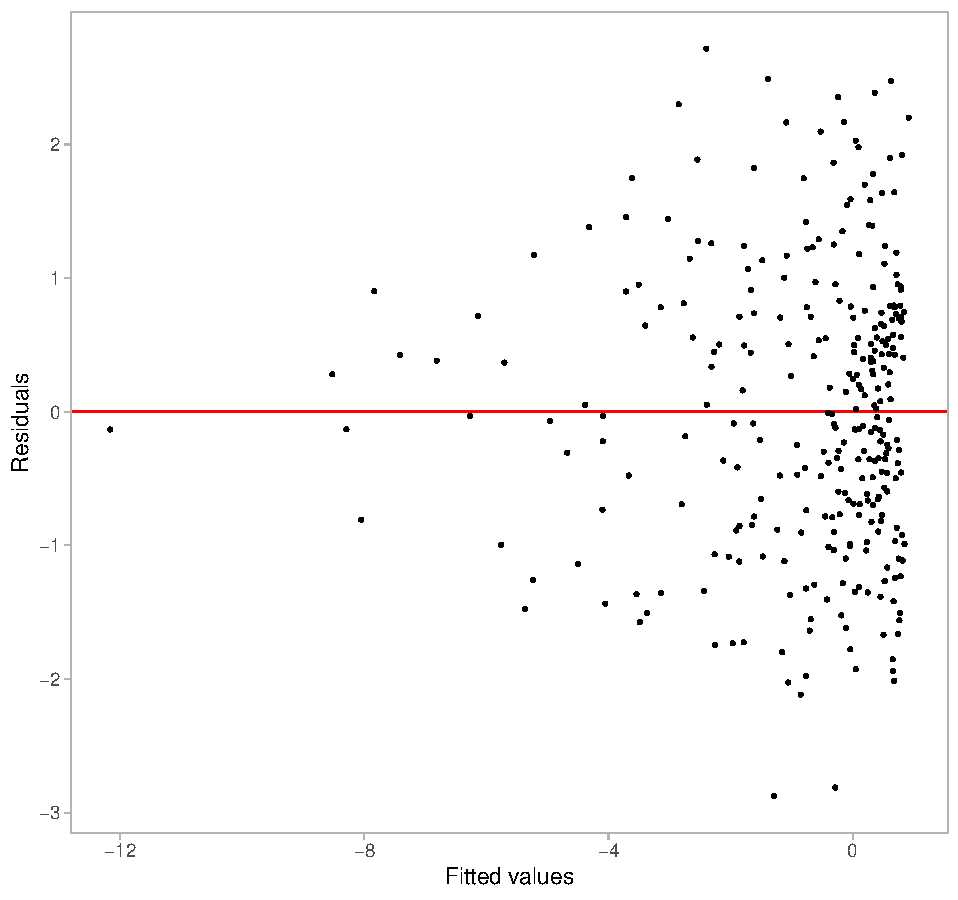
\includegraphics[width=1\linewidth]{paper_files/figure-latex/false-finding-1} 

}

\caption{An example residual vs fitted values plot (red line indicates 0). The vertical spread of the data points varies with the fitted values. This often indicates the existence of heteroskedasticity. The Breusch-Pagan test rejects this residual plot at 95\% significance level ($p\text{-value} = 0.046$).}\label{fig:false-finding}
\end{figure}

\hypertarget{methodology}{%
\section{Methodology}\label{methodology}}

\hypertarget{different-possible-configurations-of-the-model-formula}{%
\subsection{Different possible configurations of the model
formula}\label{different-possible-configurations-of-the-model-formula}}

There are various configurations of the computer vision model that can
be used to assess residual plots. We discuss these configurations below
based on two key components of the model formula: the input and the
output format.

\hypertarget{input-formats}{%
\subsubsection{Input formats}\label{input-formats}}

Deep learning models are in general very sensitive to the input data.
The quality and relevance of the input data greatly influence the
model's capacity to generate insightful and meaningful results. There
are several designs of the input format can be considered.

A straightforward design involves feeding a vector of residuals along
with a vector of fitted values, essentially providing all the necessary
information for creating a residuals vs fitted values plot. However, a
drawback of this method is the dynamic input size, which changes based
on the number of observations. For modern computer vision models
implemented in mainstream software like TensorFlow
\citep{abadi2016tensorflow}, the input shape is typically fixed. One
solution is to pad the input vectors with leading or trailing zeros when
the input tensor expects longer vectors, but it may fail if the input
vector surpasses the designed length. Another strategy is to summarize
the residuals and fitted values separately using histograms and utilize
the counts as the input. By controlling the number of bins in the
histograms, it becomes possible to provide fixed-length input vectors.
Still, since histograms only capture the marginal distribution of
residuals and fitted values respectively, they can not be used to
differentiate visual patterns with same marginal distributions but
different joint distributions.

Another design involves using an image as input. The primary advantage
of this design, as opposed to the vector format, is the availability of
the existing and sophisticated image processing architectures developed
over the years, such as the VGG16 architecture proposed in
\citet{simonyan2014very}. These architectures can effectively capture
and summarize spatial information from nearby pixels, which is less
straightforward with vector input. The main considerations are the image
resolution and the aesthetics of the residual plot. In general, higher
resolution provides more information to the model but comes with the
trade-off of increased complexity and greater difficulty in training. As
for the aesthetics of the residual plot, a practical solution is to
consistently present residual plots in the same style to the model. This
implies that the model can not accept arbitrary images as input but
requires the use of the same pre-processing pipeline to convert
residuals and fitted values into a standardized-style residual plot.

Providing multiple residual plots to the model, such as a pair of plots,
a triplet or a lineup is also a possible option.
\citet{chopra2005learning} have shown that computer vision models
designed for image comparison can assess whether a pair of images are
similar or dissimilar. Applied to our specific problem, we can define
null plots of a fitted regression model to be similar to each other,
while considering actual residual plots to be distinct from null plots
of any fitted regression model. A triplet constitutes a set of three
images, denoted as \(image_1\), \(image_2\) and \(image_3\). It is often
used to predict whether \(image_2\) or \(image_3\) is more similar to
\(image_1\), proving particularly useful for establishing rankings
between samples. For this setup, we can apply the same criteria to
define similarity between images. However, it is important to note that
these two approaches usually require additional considerations regarding
the loss function and, at times, non-standard training processes due to
shared weights between different convolutional blocks.

Presenting a lineup to a model aligns closely with the lineup protocol.
However, as the number of residual plots in a lineup increases, the
resolution of the input image grows rapidly, posing challenges in
training the model. We experimented with this approach in a pilot study,
but the performance of the trained model was sub-optimal.

We did not explore all the mentioned input formats due the considerable
costs associated with data preparation and model training. Considering
the implementation cost and the interpretability of the model, we
settled on the single residual plot input format.

\hypertarget{output-formats}{%
\subsubsection{Output formats}\label{output-formats}}

Given that the input is a single residual plot represented as a
fixed-resolution image, the output from the computer vision model can
take one of two forms: binary or numeric. This choice determines whether
the model belongs to a classification model or a regression model. The
binary outcome encoded as \(0\) and \(1\) could be used to represent
whether the input image is a null plot, or whether the input image would
be rejected in a visual test conducted by humans. Training a model
following the latter option requires data from prior human subject
experiments, presenting difficulties in controlling the quality of data
due to variations in experimental settings across different studies.
Additionally, some visual inference experiments are unrelated to linear
regression models or residual plot diagnostics, resulting in a limited
amount of available training data.

Alternatively, the output could be a meaningful and interpretable
numerical measure useful for assessing residual plots, such as the
strength of suspicious visual patterns reflecting the extent of model
violations and the difficulty index for identifying whether a residual
plot has no issues. However, these numeric measures are often informally
used in daily communication but are not typically formalized or
rigorously defined. For the purpose of training a model, this numeric
measure has to be quantifiable.

In this study, we chose to define and use a distance measure to quantify
the difference between the residual plot and the null plots.
\citet{vo2016localizing} have also demonstrated that defining a proper
distance between images can enhance the matching accuracy in image
search compared to a binary outcome model.

\hypertarget{distance-from-the-good-residual-plots}{%
\subsection{Distance from the good residual
plots}\label{distance-from-the-good-residual-plots}}

In a visual test, the observer will be asked to choose one or more plots
that stand out as most distinct from others in a given lineup. To
develop a computer vision model for assessing residual plots within the
visual inference framework, it is important to precisely define a
numerical measure of ``difference'' or ``distance'' between plots. This
distance can take the form of a basic statistical operation on pixels,
such as the sum of square differences. Alternatively, it could involve
established image similarity metrics like the Structural Similarity
Index Measure \citep{wang2004image}. The challenge lies in the fact that
metrics tailored for image comparison may not be suitable for evaluating
data plots, where only essential plot elements require assessment
\citep{chowdhury2018measuring}. Furthermore, scagnostics mentioned in
Section \ref{introduction} could be used to construct distance metrics
for residual plots comparison, but the functional form still needs to be
carefully refined to accurately reflect the extent of the violations.

\hypertarget{residual-distribution}{%
\subsubsection{Residual distribution}\label{residual-distribution}}

The distance measure proposed in this study takes into account the fact
that we tried to measure how different a residual plot is from a good
residual plot, or in other words, how different a given fitted
regression model is from a correctly specified model. For the classical
normal linear regression model, residuals \(\boldsymbol{e}\) are derived
from the fitted values \(\hat{\boldsymbol{y}}\) and observed values
\(\boldsymbol{y}\). Suppose the data generating process is known and the
regression model is correctly specified, by the Frisch-Waugh-Lowell
theorem \citep{frisch1933partial}, residuals \(\boldsymbol{e}\) can also
be treated as random variables and written as a linear transformation of
the error \(\boldsymbol{\varepsilon}\) formulated as
\(\boldsymbol{e} = \boldsymbol{R}\boldsymbol{\varepsilon}\), where
\(\boldsymbol{R}=\boldsymbol{I}_n -\boldsymbol{X}(\boldsymbol{X}'\boldsymbol{X})^{-1}\boldsymbol{X}'\)
is the residual operator and an idempotent matrix, \(\boldsymbol{X}\) is
the design matrix, \(\boldsymbol{I}_n\) is a \(n\) by \(n\) identity
matrix, and \(n\) is the number of observations.

One of the assumptions of the classical normal linear regression model
is the error \(\boldsymbol{\varepsilon}\) follows a multivariate normal
distribution with zero mean and constant variance, i.e.,
\(\boldsymbol{\varepsilon} \sim N(\boldsymbol{0}_n,\sigma^2\boldsymbol{I}_n)\).
It can be known that residuals \(\boldsymbol{e}\) also follow a certain
probability distribution transformed from the multivariate normal
distribution, which will be denoted as \(Q\). This reference
distribution \(Q\) summarizes what good residuals should follow given
the design matrix \(\boldsymbol{X}\) is known and fixed.

In ordinary least square, the minimization of the sum of square
residuals implies \(\sum_{i=1}^{n} e_i = 0\), making any residual value
to be a linear combination of the remaining \(n - 1\) residuals. This
effectively means \(\text{rank}(\boldsymbol{R}) = n - 1 < n\) and \(Q\)
is a degenerate multivariate distribution. To capture the
characteristics of \(Q\), such as moments, we can simulate a large
numbers of \(\boldsymbol{\varepsilon}\) and transform it to
\(\boldsymbol{e}\) to get the empirical estimates. For simplicity, in
this study, we replaced the variance-covariance matrix of residuals
\(\text{cov}(\boldsymbol{e}, \boldsymbol{e}) = \boldsymbol{R}\sigma^2\boldsymbol{R}' = \boldsymbol{R}\sigma^2\)
with a full-rank diagonal matrix
\(\text{diag}(\boldsymbol{R}\sigma^2)\), where \(\text{diag}(.)\) sets
the non-diagonal entries of a matrix to zeros. The resulting
distribution for \(\boldsymbol{Q}\) is
\(N(\boldsymbol{0}_n, \text{diag}(\boldsymbol{R}\sigma^2))\).

Distribution \(Q\) is derived from the correctly specified model.
However, if the model is misspecified, then the actual distribution of
residuals denoted as \(P\), will be different from \(Q\). For example,
if the data generating process contains variables correlated with any
column of \(\boldsymbol{X}\) but not included in \(\boldsymbol{X}\),
causing an omitted variable problem, \(P\) will be different from \(Q\)
because the residual operator obtained from the fitted regression model
will not be the same as \(\boldsymbol{R}\). Besides, if the
\(\boldsymbol{\varepsilon}\) follows a non-normal distribution such as a
multivariate log-normal distribution, \(P\) will usually be skewed and
has a long tail.

\hypertarget{kullback-leibler-divergence-of-p-from-q}{%
\subsubsection{\texorpdfstring{Kullback-Leibler divergence of \(P\) from
\(Q\)}{Kullback-Leibler divergence of P from Q}}\label{kullback-leibler-divergence-of-p-from-q}}

Define a proper distance between distributions is usually easier than
define a proper distance between data plots. Given the actual residual
distribution \(Q\) and the reference residual distribution \(P\), we
used a distance measure based on Kullback-Leibler divergence
\citep{kullback1951information} to quantify the difference between two
distributions

\begin{align}
\label{eq:kl-0}
D &= \log\left(1 + D_{KL}\right), \\
\label{eq:kl-1}
D_{KL} &= \int_{\mathbb{R}^{n}}\log\frac{p(\boldsymbol{e})}{q(\boldsymbol{e})}p(\boldsymbol{e})d\boldsymbol{e},
\end{align}

\noindent where \(p(.)\) is the probability density function for
distribution \(P\), and \(q(.)\) is the probability density function for
distribution \(Q\).

This distance measure was first proposed in \citet{li2023plot}. It was
mainly designed for measuring the effect size of non-linearity and
heteroskedasticity in a residual plot. \citet{li2023plot} have showed
that, for a classical normal linear regression model that omits a
necessary higher-order predictors \(\boldsymbol{Z}\), and incorrectly
assumes
\(\boldsymbol{\varepsilon} \sim N(\boldsymbol{0}_n,\sigma^2\boldsymbol{I}_n)\)
while in fact
\(\boldsymbol{\varepsilon} \sim N(\boldsymbol{0}_n, \boldsymbol{V})\)
with \(\boldsymbol{V}\) being an arbitrary symmetric positive
semi-definite matrix, \(Q\) can be represented as
\(N(\boldsymbol{R}\boldsymbol{Z}\boldsymbol{\beta}_z, \text{diag}(\boldsymbol{R}\boldsymbol{V}\boldsymbol{R}))\).
Note that the variance-covariance matrix is replaced with the diagonal
matrix to ensure it is a full-rank matrix.

Since both \(P\) and \(Q\) are adjusted to be multivariate normal
distributions, equation \ref{eq:kl-1} can be further expanded to

\begin{align}
\label{eq:kl-2}
D_{KL} &= \frac{1}{2}\left(\log\frac{|\text{diag}(\boldsymbol{W})|}{|\text{diag}(\boldsymbol{R}\sigma^2)|} - n + \text{tr}(\text{diag}(\boldsymbol{W})^{-1}\text{diag}(\boldsymbol{R}\sigma^2)) + \boldsymbol{\mu}_z'(\text{diag}(\boldsymbol{W}))^{-1}\boldsymbol{\mu}_z\right),
\end{align}

\noindent where
\(\boldsymbol{\mu}_z = \boldsymbol{R}\boldsymbol{Z}\boldsymbol{\beta}_z\),
and \(\boldsymbol{W} = \boldsymbol{R}\boldsymbol{V}\boldsymbol{R}\). The
assumed error variance \(\sigma^2\) is set to be
\(\text{tr}(\boldsymbol{V})/n\), which is the expectation of the
estimated variance.

\hypertarget{evaluation-of-kullback-leibler-divergence-for-non-normal-p}{%
\subsubsection{\texorpdfstring{Evaluation of Kullback-Leibler divergence
for non-normal
\(P\)}{Evaluation of Kullback-Leibler divergence for non-normal P}}\label{evaluation-of-kullback-leibler-divergence-for-non-normal-p}}

For non-normal error \(\boldsymbol{\varepsilon}\), the actual residual
distribution \(P\) is unlikely to be a multivariate normal distribution.
Thus, equation \ref{eq:kl-2} given in \citet{li2023plot} will not be
applicable to models violating the normality assumption.

To evaluate the Kullback-Leibler divergence of non-normal \(P\) from
\(Q\), the fallback is to solve equation \ref{eq:kl-1} numerically.
However, since \(\boldsymbol{e}\) is a linear transformation of
non-normal random variables, it is very common that the general form of
\(P\) is unknown, meaning that we can not easily compute
\(p(\boldsymbol{e})\) using a well-known probability density function.
Additionally, even if \(p(\boldsymbol{e})\) can be calculated for any
\(\boldsymbol{e} \in \mathbb{R}^n\), it will be very difficult to do
numerical integration over the \(n\) dimensional space, because \(n\)
could be potentially very large.

In order to approximate \(D_{KL}\) in a practically computable manner,
the elements of \(\boldsymbol{e}\) are assumed to be independent of each
other. This assumption solves both of the issues mentioned above. First,
we no longer need to integrate over \(n\) random variables. The result
of equation \ref{eq:kl-1} is now the sum of the Kullback-Leibler
divergence evaluated for each individual residual thanks for the
independence assumption. Second, it is not required to know the joint
probability density \(p(\boldsymbol{e})\) any more. Instead, the
evaluation of Kullback-Leibler divergence for an individual residual
relies on the knowledge of the marginal density \(p_i(e_i)\), where
\(e_i\) is the \(i\)-th residual for \(i = 1, ..., n\). This is much
easier to approximate through simulation. It is also worth mentioning
that this independence assumption generally will not hold, since
\(\text{cov}(e_i, e_j) \neq 0\) if \(\boldsymbol{R}_{ij} \neq 0\) for
any \(1 \leq i < j \leq n\), but its existence is essential for reducing
the computational cost.

Given \(\boldsymbol{X}\) and \(\boldsymbol{\beta}\), the algorithm for
approximating equation \ref{eq:kl-1} starts from simulating \(m\) sets
of observed values \(\boldsymbol{y}\) according to the data generating
process. The observed values are stored in a matrix \(\boldsymbol{A}\)
with \(n\) rows and \(m\) columns, where each column of
\(\boldsymbol{A}\) is a set of observed values. Then, we can get \(m\)
sets of realized values of \(\boldsymbol{e}\) stored in the matrix
\(\boldsymbol{B}\) by applying the residual operator
\(\boldsymbol{B} = \boldsymbol{R}\boldsymbol{A}\). Furthermore, kernel
density estimation (KDE) with Gaussian kernel and optimal bandwidth
selected by the Silverman's rule of thumb \citep{silverman2018density}
is applied on each row of \(B\) to estimate \(p_i(e_i)\) for
\(i = 1, ..., n\). The KDE computation can be done by the
\texttt{density} function in R.

Since the Kullback-Leibler divergence can be viewed as the expectation
of the log-likelihood ratio between distribution \(P\) and distribution
\(Q\) evaluated on distribution \(P\), we can reuse the simulated
residuals in matrix \(\boldsymbol{B}\) to estimate the expectation by
the sample mean. With the independence assumption, for non-normal \(P\),
\(D_{KL}\) can be approximated by

\begin{align}
\label{eq:kl-3}
D_{KL} &\approx \sum_{i = 1}^{n} \hat{D}_{KL}^{(i)}, \\
\hat{D}_{KL}^{(i)} &= \frac{1}{m}\sum_{j = 1}^{m} log\frac{\hat{p_i}(B_{ij})}{q(B_{ij})},
\end{align}

\noindent where \(\hat{D}_{KL}^{(i)}\) is the estimator of the
Kullback-Leibler divergence for an individual residual \(e_i\),
\(B_{ij}\) is the \(i\)-th row and \(j\)-th column entry of the matrix
\(B\), \(\hat{p_i}(.)\) is the kernel density estimator of \(p_i(.)\),
\(q(.)\) is the normal density function with mean zero and an assumed
variance estimated as
\(\widehat{\sigma^2} = \sum_{b \in vec(B)}(b - \sum_{b \in vec(B)} b/nm)^2/(nm - 1)\),
and \(vec(.)\) is the vectorization operator which turns a
\(n \times m\) matrix into a \(nm \times 1\) column vector by stacking
the columns of the matrix on top of each other.

\hypertarget{approximation-of-the-distance-measure}{%
\subsubsection{Approximation of the distance
measure}\label{approximation-of-the-distance-measure}}

In the previous sections, we have defined a distance measure given in
equation \ref{eq:kl-0} for quantifying the difference between the actual
residual distribution \(P\) and an ideal reference distribution \(Q\).
You may have noticed that this distance measure can only be computed
when the data generating process is known. In reality, we often have no
knowledge about the data generating process, otherwise we do not need to
fit a linear regression model in the first place.

We tried to train a computer vision model to approximate this distance
measure with a residual plot. Let \(D\) be the result of equation
\ref{eq:kl-0}, and our estimator \(\hat{D}\) is formulated as

\begin{equation}
\label{eq:d-approx}
\hat{D} = f_{CV}(V_{h \times w}(\boldsymbol{e}, \hat{\boldsymbol{y}})),
\end{equation}

\noindent where \(V_{h \times w}(.)\) is a plotting function that saves
a residuals vs fitted values plot with fixed aesthetic as an image with
\(h \times w\) pixels and three colour channels, \(f_{CV}(.)\) is a
computer vision model which takes an \(h \times w\) image as input and
predicts the distance in the domain \([0, +\infty)\).

With the approximated distance \(\hat{D}\), we will be able to know how
different the underlying distribution of the residuals is from a good
residual distribution. The approximated distance \(\hat{D}\) can also be
used as an index of the model violations. It also provides information
for the strength of the visual signal embedded in the residual plot.

The approximated distance \(\hat{D}\) is not expected to be the same as
the original distance \(D\). This is largely because information
contained in a single residual plot is limited and it may not be able to
summarise all the important characteristics of the residual
distribution. For a given residual distribution \(P\), we can generate
many different residual plots. Some of them share similar visual
patterns, but some of them could be visually very different from the
rest, especially for regression models with small \(n\). This suggests
the error of the approximation will vary depends on whether the observed
residual plot is representative or not.

\hypertarget{approximated-distance-as-an-model-violations-index-mvi}{%
\subsubsection{Approximated distance as an Model Violations Index
(MVI)}\label{approximated-distance-as-an-model-violations-index-mvi}}

In Section \ref{output-formats}, we discuss the output formats of the
computer vision model presented in this paper. One notable advantage
highlighted is its interpretability. The approximated distance
\(\hat{D}\) is an estimator of the difference between the actual
residual distribution and the reference residual distribution. This
difference primarily arises from deviations in model assumptions. The
magnitude of \(D\) directly reflects the degree of these deviations,
thus making \(\hat{D}\) instrumental in forming a model violation index.

Note that since the Kullback-Leibler divergence could be affected by the
number of random variables involved in the evaluation. In general, more
observations will result in greater distance \(D\). This does not mean
\(\hat{D}\) can not correctly represent the extent of the model
violations since more observations in a residual plot usually lead to
stronger visual signal strength as the underlying visual patterns will
have higher chance to be revealed except for cases like serious
overlapping. For the same data generating process, \(D\) usually grows
logarithmically as the number of observations increases. This is because
\(D = \text{log}(1 + D_{KL})\), and
\(D_{KL} = \sum_{i=1}^{n}D_{KL}^{(i)}\) under the independence
assumption.

Note that the Kullback-Leibler divergence might be influenced by the
number of random variables involved in its evaluation. Generally, a
larger number of observations will lead to a greater distance \(D\).
However, this does not imply that \(\hat{D}\) fails to accurately
represent the extent of model violations. In fact, when examining
residual plots with more observations, we often observe a stronger
visual signal strength, as the underlying patterns are more likely to be
revealed, except in cases of significant overlapping.

For a consistent data generating process, \(D\) typically increases
logarithmically with the number of observations. This behaviour comes
from the relationship \(D = \text{log}(1 + D_{KL})\), where
\(D_{KL} = \sum_{i=1}^{n}D_{KL}^{(i)}\) under the assumption of
independence.

Therefore, the Model Violations Index (MVI) can be proposed as

\begin{equation}
\label{eq:mvi}
\text{MVI} = C + \hat{D} - log(n),
\end{equation}

\noindent where \(C\) is a large enough constant keeping the result
positive.

\hypertarget{statistical-testing-based-on-the-approximated-distance}{%
\subsection{Statistical testing based on the approximated
distance}\label{statistical-testing-based-on-the-approximated-distance}}

\hypertarget{null-distribution-of-the-approximated-distance}{%
\subsubsection{Null distribution of the approximated
distance}\label{null-distribution-of-the-approximated-distance}}

Theoretically, the distance \(D\) for a correctly specified model is
\(0\), because \(P\) will be the same as \(Q\). However, the computer
vision model may not necessary predict \(0\) for a null plot. Using
Figure \ref{fig:false-finding} as an example, it contains a visual
pattern which is an indication of heteroskedasticity. We would not
expect the model to be able to magically tell if the suspicious pattern
is caused by the skewed distribution of the fitted values or the
existence of heteroskedasticity. Additionally, some null plots could
have outliers or strong visual patterns due to randomness, and a
reasonable model will try to summarise those information into the
prediction, resulting in \(\hat{D} > 0\).

This property is not an issue if \(\hat{D} \gg 0\) for which the visual
signal of the residual plot is very strong, and we usually do not need
any further examination of the significance of the result. However, if
the visual pattern is weak or moderate, having \(\hat{D}\) will not be
sufficient to determine if \(H_0\) should be rejected.

To solve this issue while aligning with the principle of visual
inference, \(\hat{D}\) can be viewed as a test statistic. And the null
distribution of this statistic can be approximated by the empirical
distribution of \(\hat{D}_{null}\), where \(\hat{D}_{null}\) is the
approximated distance for a null plot simulated from the fitted
regression model. The approximation of the distribution involves
applying the residual rotation technique \citep{buja2009statistical} on
the fitted regression model to obtain null residuals. The null residuals
are then used to make null plots and fed into the computer vision model
to get predictions. The empirical distribution is constructed with the
approximated distance.

There are two types of error associated with the approximation of the
null distribution. These include the sampling error and the estimation
error for model parameters. Increasing the number of null plots within
the distribution approximation can effectively reduce sampling error.
However, the estimation error for model parameters remains irreducible.
The residual rotation technique operates under the assumption of a
correct fitted model, using the estimated variance instead of the
unknown true variance to rescale rotated residuals. Consequently, under
\(H_0\), the true distribution of \(\hat{D}_{null}\) will slightly
deviate from the approximated null distribution.

\hypertarget{estimation-of-quantiles-of-the-null-distribution}{%
\subsubsection{Estimation of quantiles of the null
distribution}\label{estimation-of-quantiles-of-the-null-distribution}}

Let \(\hat{D}_{null}^{(i)}\) be the approximated distance of the
\(i\)-th null plots, where \(i = 1,...,n_{null}\) and
\(n_{null} \in \mathbb{N}^+\) is a sufficiently large number. Quantiles
of the null distribution can then be estimated using the sample
quantiles available in statistical software such as R. The details of
the sample quantile computation can be found in
\citet{hyndman1996sample}. In statistical testing, analysts often care
about certain quantiles of the null distribution, such as the 90\%
quantile, the 95\% quantile and the 99\% quantile. These quantiles are
used as critical values to decide if \(H_0\) needs to be rejected. For
example, if \(\hat{D}\) is greater than and equal to the 95\% sample
quantile \(Q_{null}(0.95)\), we could say the approximated distance for
the actual residual plot is significantly different from the
approximated distance for null plots with 95\% significance level. Based
on our experience, in order to get a stable estimate of the 95\%
quantile, \(n_{null}\) usually needs to be at least \(100\). And if the
null distribution has a long tail, more null plots will be needed.
Alternatively, a p-value can be used to represents the probability of
observing an event equally or more extreme than the given event under
\(H_0\), and it can be estimated by
\(1/m\sum_{i=1}^{n_{null}}I\left(\hat{D}_{null}^{(i)} \geq \hat{D}\right)\).

If precision in sample quantiles is not the main priority, using a
pre-calculated table of quantiles is an available option. Such a table
offers pre-determined quantiles for a specified number of observations.
It is generated by assessing numerous null plots derived from various
simulated regression models and averaging them. Essentially, this shifts
the computational burden from the user to the developer.

\hypertarget{bootstrapping-the-approximated-distance}{%
\subsubsection{Bootstrapping the approximated
distance}\label{bootstrapping-the-approximated-distance}}

Bootstrap is often employed in linear regression when conducting
inference for estimated parameters. It is typically done by sampling
individual cases with replacement and refitting the regression model. If
the observed data accurately reflects the true distribution of the
population, the bootstrapped estimates can be used to measure the
variability of the parameter estimate without making strong
distributional assumptions about the data generating process.

Similarly, bootstrap can be applied on the approximated distance
\(\hat{D}\). For each refitted model \(M_{boot}^{(i)}\), there will be
an associated residual plot \(V_{boot}^{(i)}\) which can be fed into the
computer vision model to obtain \(\hat{D}_{boot}^{(i)}\), where
\(i = 1,...,n_{boot}\), and \(n_{boot}\) is the number of bootstrapped
samples. If we are interested in the variation of \(\hat{D}\), we can
use \(\hat{D}_{boot}^{(i)}\) to estimate a confidence interval.

Alternatively, since each \(M_{boot}^{(i)}\) has a set of estimated
coefficients \(\hat{\boldsymbol{\beta}}_{boot}^{(i)}\) and an estimated
variance \(\hat{\sigma^2}_{boot}^{(i)}\), a new approximated null
distribution can be construed and the corresponding 95\% sample quantile
\(Q_{boot}^{(i)}(0.95)\) can be computed. Then, if
\(\hat{D}_{boot}^{(i)} \geq Q_{boot}^{(i)}(0.95)\), \(H_0\) will be
rejected for \(M_{boot}^{(i)}\). The ratio of rejected
\(M_{boot}^{(i)}\) among all the refitted models provides an indication
of how often the assumed regression model are considered to be incorrect
if the data can be obtained repetitively from the same data generating
process. But this approach is computationally very expensive because it
requires \(n_{boot} \times n_{null}\) times of residual plot assessment.
In practice, \(Q_{null}(0.95)\) can be used to replace
\(Q_{boot}^{(i)}(0.95)\) in the computation.

\hypertarget{generation-of-training-data}{%
\subsection{Generation of training
data}\label{generation-of-training-data}}

\hypertarget{data-generating-process}{%
\subsubsection{Data generating process}\label{data-generating-process}}

While observational data is frequently employed in training models for
real-world applications, the data generating process of observational
data often remains unknown, making computation for our target variable
\(D\) unattainable. Consequently, the computer vision models developed
in this study were trained using synthetic data. This approach provided
us with precise label annotations. Additionally, it ensured a large and
diverse training dataset, as we had control over the data generating
process, and the simulation of the training data was relatively
cost-effective.

We have incorporated three types of residual departures of linear
regression model in the training data, including non-linearity,
heteroskedasticity and non-normality. All three departures can be
summarised by the data generating process formulated as

\begin{align}
\label{eq:data-sim}
\boldsymbol{y} &= \boldsymbol{1}_n + \boldsymbol{x}_1 + \beta_1\boldsymbol{x}_2 + \beta_2(\boldsymbol{z} + \beta_1\boldsymbol{w}) + \boldsymbol{k} \odot \boldsymbol{\varepsilon}, \\
\boldsymbol{z} &= \text{He}_j(g(\boldsymbol{x}_1, 2)), \\
\boldsymbol{w} &= \text{He}_j(g(\boldsymbol{x}_2, 2)), \\
\boldsymbol{k} &= \sqrt{\boldsymbol{1}_n + b(2 - |a|)(\boldsymbol{x}_1 + \beta_1\boldsymbol{x}_2 - a\boldsymbol{1}_n)^2},
\end{align}

\noindent where \(\boldsymbol{y}\), \(\boldsymbol{x}_1\),
\(\boldsymbol{x}_2\), \(\boldsymbol{z}\), \(\boldsymbol{w}\),
\(\boldsymbol{k}\) and \(\boldsymbol{\varepsilon}\) are vectors of size
\(n\), \(\boldsymbol{1}_n\) is a vector of ones of size \(n\),
\(\boldsymbol{x}_1\) and \(\boldsymbol{x}_2\) are two independent
predictors, \(\text{He}_j(.)\) is the \(j\)th-order probabilist's
Hermite polynomials \citep{hermite1864nouveau}, the \(\sqrt{(.)}\) and
\((.)^2\) operators are element-wise operators, \(\odot\) is the
Hadamard product, and \(g(., k)\) is a scaling function to enforce the
support of the random vector to be \([-k, k]^n\) defined as

\[g(\boldsymbol{x}, k) = 2k \cdot \frac{\boldsymbol{x} - x_{min}\boldsymbol{1}_n}{x_{max} - x_{min}} - k\boldsymbol{1}_n,~for~k > 0,\]
\noindent where \(x_{min} = \underset{i \in \{ 1,...,n\}}{min} x_i\),
\(x_{max} = \underset{i \in \{ 1,...,n\}}{max} x_i\) and \(x_i\) is the
\(i\)-th entry of \(\boldsymbol{x}\).

\begin{table}

\caption{\label{tab:factor}Factors used in the data generating process for synthetic data simulation. Factor $j$ and $a$ controls the non-linearity shape and the heteroskedasticity shape respectively. Factor $b$, $\sigma_\varepsilon$ and $n$ control the signal strength. Factor $\text{dist}_\varepsilon$, $\text{dist}_{x1}$ and $\text{dist}_{x2}$ specifies the distribution of $\varepsilon$, $X_1$ and $X_2$ respectively.}
\centering
\begin{tabular}[t]{ll}
\toprule
Factor & Domain\\
\midrule
j & \{2, 3, ..., 18\}\\
a & {}[-1, 1]\\
b & {}[0, 100]\\
$\beta_1$ & {0, 1}\\
$\beta_2$ & {0, 1}\\
\addlinespace
$\text{dist}_\varepsilon$ & \{discrete, uniform, normal, lognormal\}\\
$\text{dist}_{x1}$ & \{discrete, uniform, normal, lognormal\}\\
$\text{dist}_{x2}$ & \{discrete, uniform, normal, lognormal\}\\
$\sigma_{\varepsilon}$ & {}[0.0625, 9]\\
$\sigma_{X1}$ & {}[0.3, 0.6]\\
\addlinespace
$\sigma_{X2}$ & {}[0.3, 0.6]\\
n & {}[50, 500]\\
\bottomrule
\end{tabular}
\end{table}

The residuals and fitted values of the fitted model were obtained by
regressing \(\boldsymbol{y}\) on \(\boldsymbol{x}_1\). If
\(\beta_1 \neq 0\), \(\boldsymbol{x}_2\) was also included in the design
matrix. This data generation process was adapted from
\citet{li2023plot}, where it was utilized to simulate residual plots
exhibiting non-linearity and heteroskedasticity visual patterns for
human subject experiments. A summary of the factors utilized in Equation
\ref{eq:data-sim} is provided in Table \ref{tab:factor}.

In Equation \ref{eq:data-sim}, \(\boldsymbol{z}\) and \(\boldsymbol{w}\)
represent higher-order terms of \(\boldsymbol{x}_1\) and
\(\boldsymbol{x}_2\), respectively. If \(\beta_2 \neq 0\), the
regression model will encounter non-linearity issues. Parameter \(j\)
serves as a shape parameter that controls the number of tuning points in
the non-linear pattern. Typically, higher values of \(j\) lead to an
increase in the number of tuning points, as illustrated in Figure
\ref{fig:different-j}.

\begin{figure}[!h]

{\centering 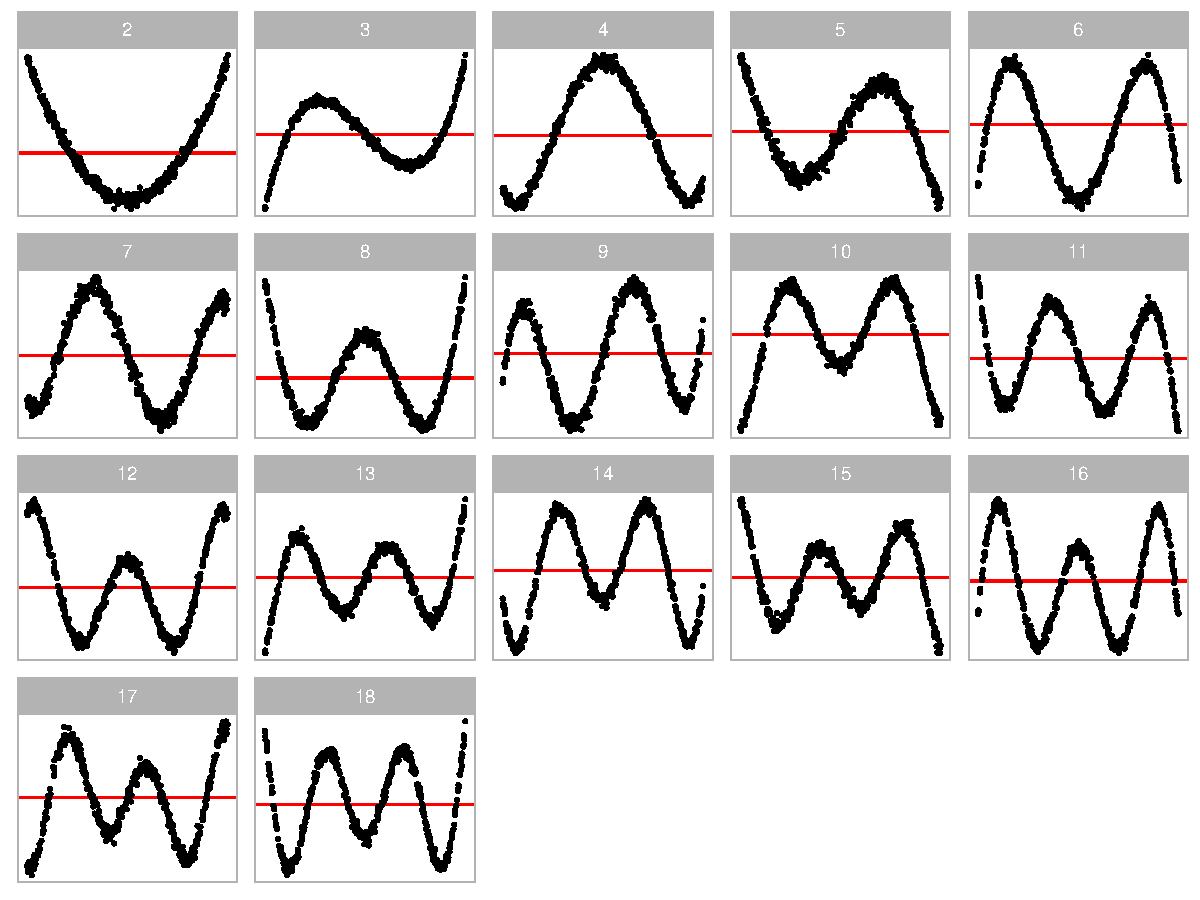
\includegraphics[width=1\linewidth]{paper_files/figure-latex/different-j-1} 

}

\caption{Non-linearity forms generated for the synthetic data simulation. The 17 shapes are generated by varying the order of polynomial given by $j$ in $He_j(.)$.}\label{fig:different-j}
\end{figure}

Additionally, Scaling factor \(\boldsymbol{k}\) directly affects the
error distribution and it is correlated with \(\boldsymbol{x}_1\) and
\(\boldsymbol{x}_2\). If \(b \neq 0\) and
\(\boldsymbol{\varepsilon} \sim N(\boldsymbol{0}_n, \sigma^2\boldsymbol{I}_n)\),
the constant variance assumption will be violated. Parameter \(a\) is a
shape parameter controlling the location of the smallest variance in a
residual plot as shown in Figure \ref{fig:different-a}.

\begin{figure}[!h]

{\centering 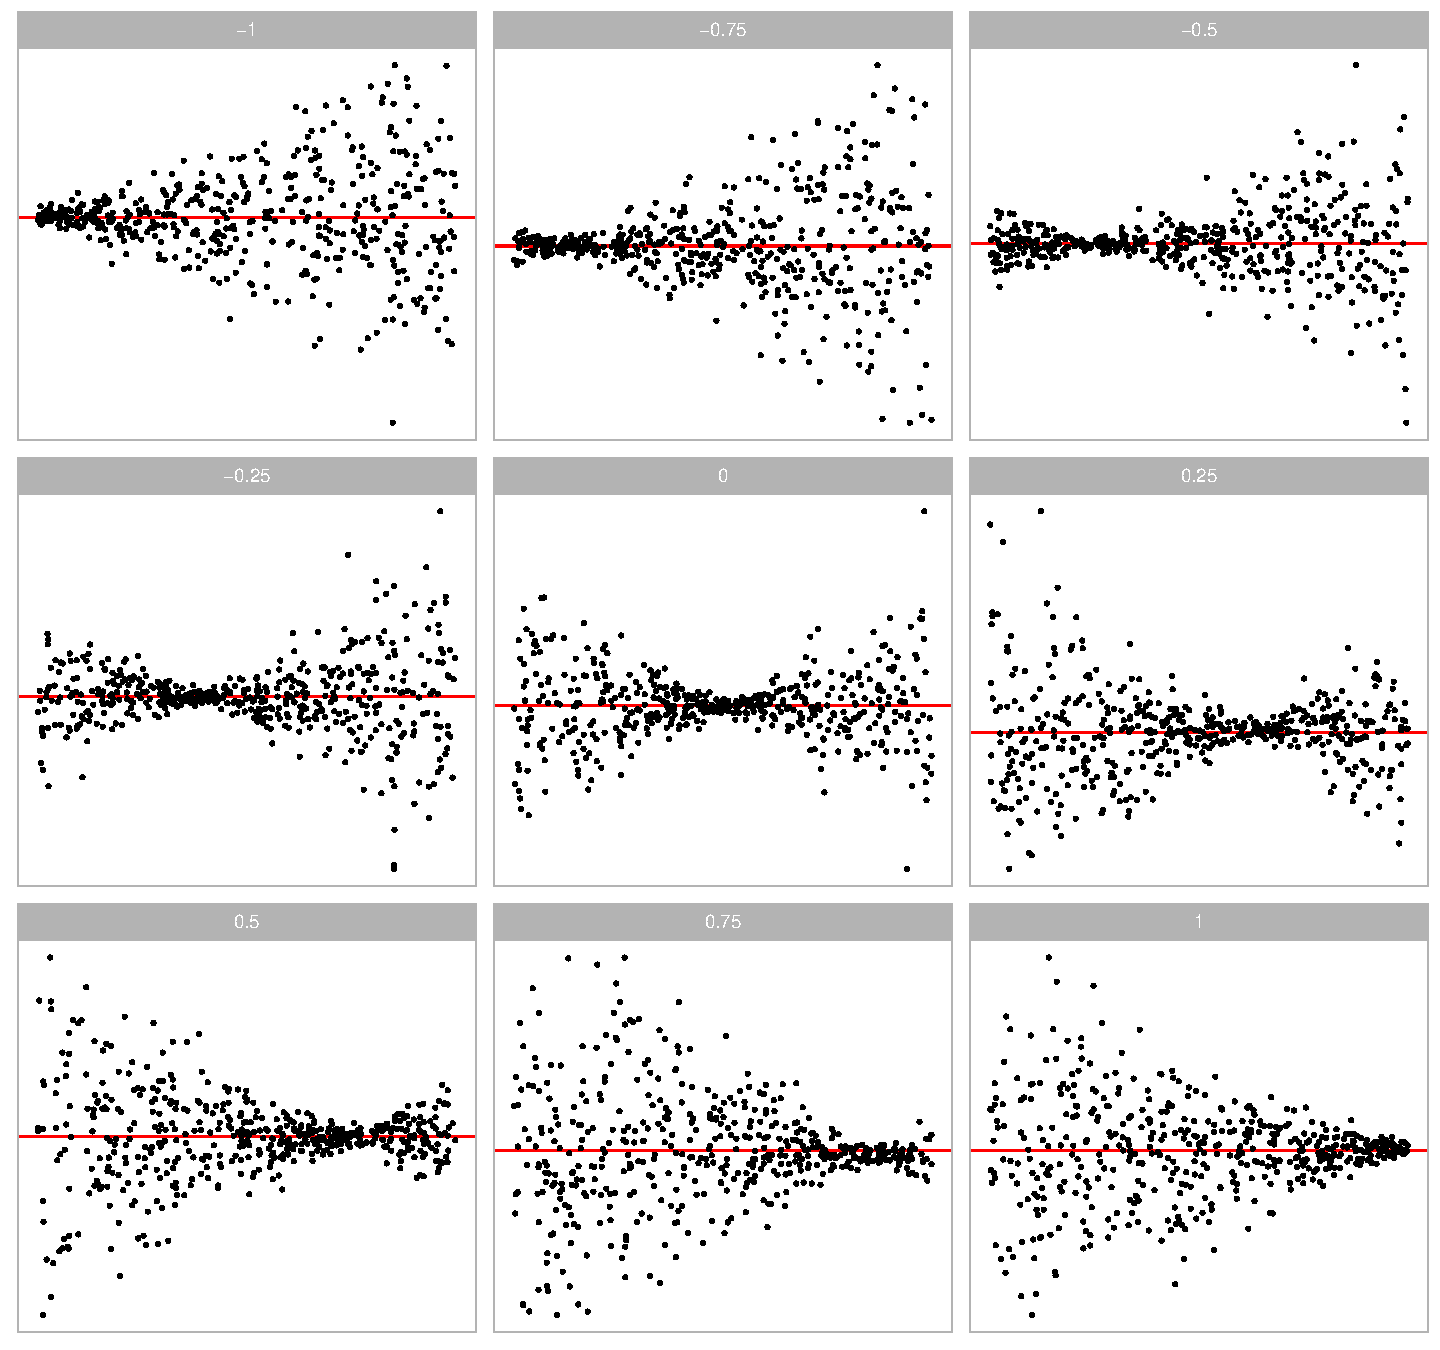
\includegraphics[width=1\linewidth]{paper_files/figure-latex/different-a-1} 

}

\caption{Heteroskedasticity forms generated for the synthetic data simulation. Different shapes are controlled by the continuous factor $a$ between -1 and 1. For $a = -1$, the residual plot exhibits a "left-triangle" shape. And for $a = 1$, the residual plot exhibits a "right-triangle" shape. }\label{fig:different-a}
\end{figure}

\begin{figure}[!h]

{\centering 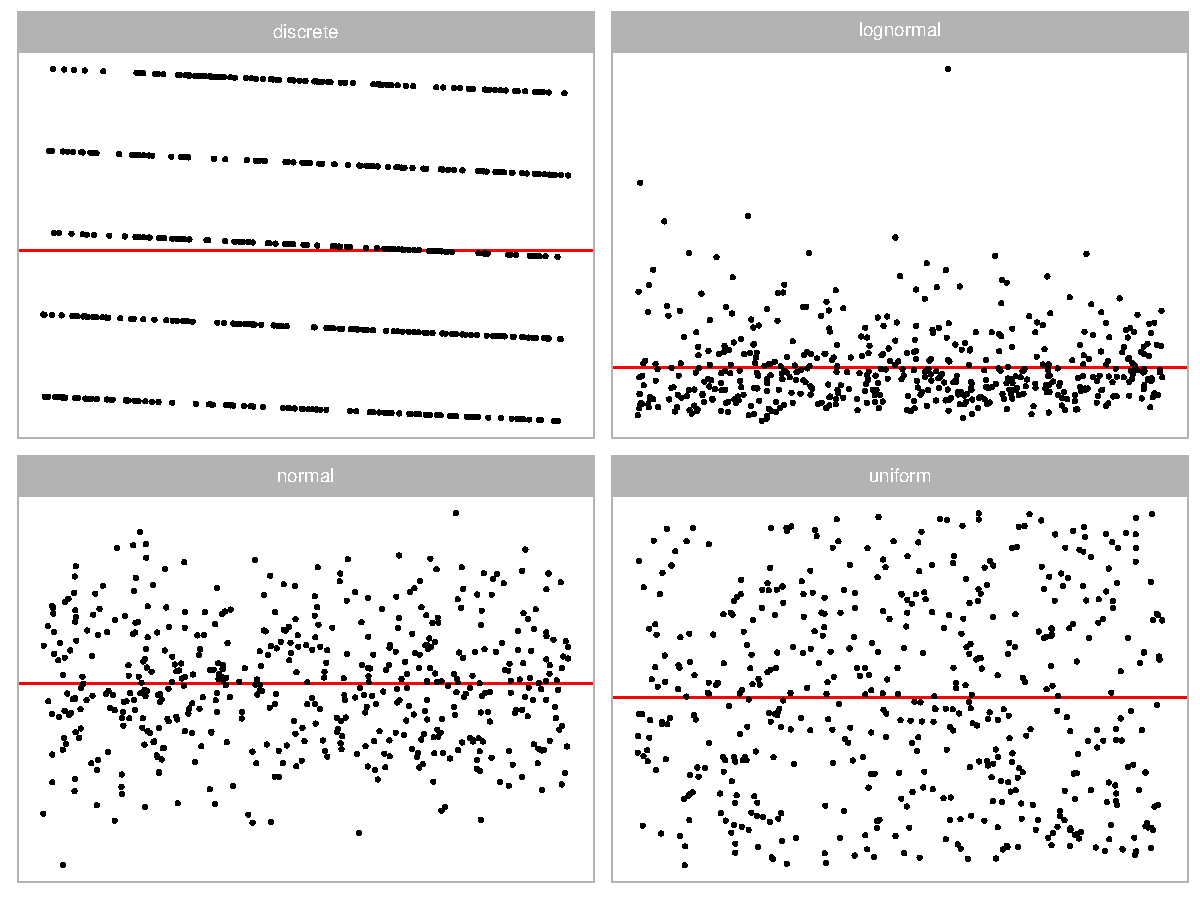
\includegraphics[width=1\linewidth]{paper_files/figure-latex/different-e-1} 

}

\caption{Non-normality forms generated for the synthetic data simulation. Four different error distributions including discrete, lognormal, normal and uniform are considered.}\label{fig:different-e}
\end{figure}

Non-normality violations arise from specifying a non-normal distribution
for \(\boldsymbol{\varepsilon}\). In the synthetic data simulation, four
distinct error distributions are considered, including discrete,
uniform, normal, and log-normal distributions, as presented in Figure
\ref{fig:different-e}. Each distribution imparts unique characteristics
to the residuals. The discrete error distribution introduces
discreteness in residuals, while the log-normal distribution typically
yields outliers. Uniform error distribution may result in residuals
filling the entire space of the residual plot. All of these
distributions exhibit visual distinctions from the normal error
distribution.

\begin{figure}[!h]

{\centering 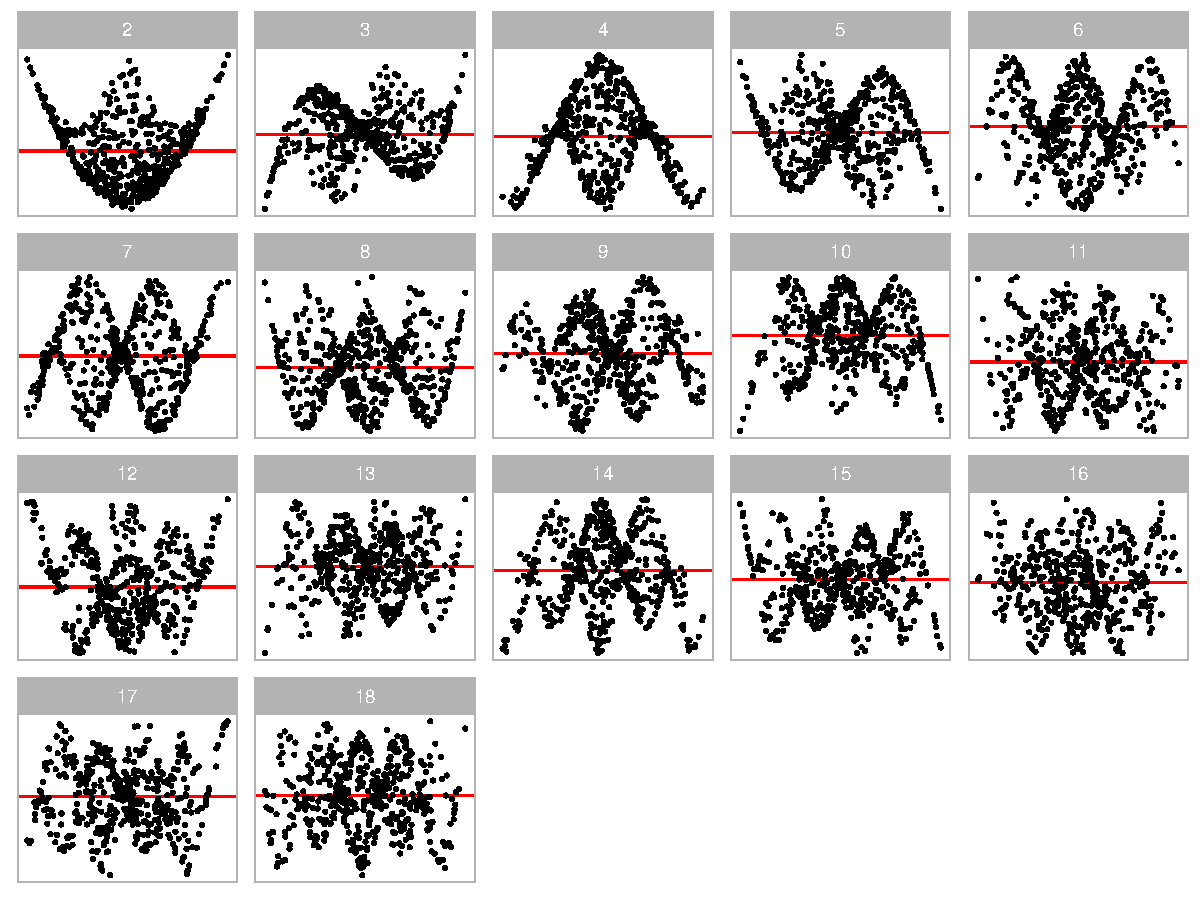
\includegraphics[width=1\linewidth]{paper_files/figure-latex/different-j-x2-1} 

}

\caption{Residual plots of multiple linear regression models with non-linearity issues. The 17 shapes are generated by varying the order of polynomial given by $j$ in $He_j(.)$. A second predictor $\boldsymbol{x}_2$ is introduced to the regression model to create complex shapes.}\label{fig:different-j-x2}
\end{figure}

\begin{figure}[!h]

{\centering 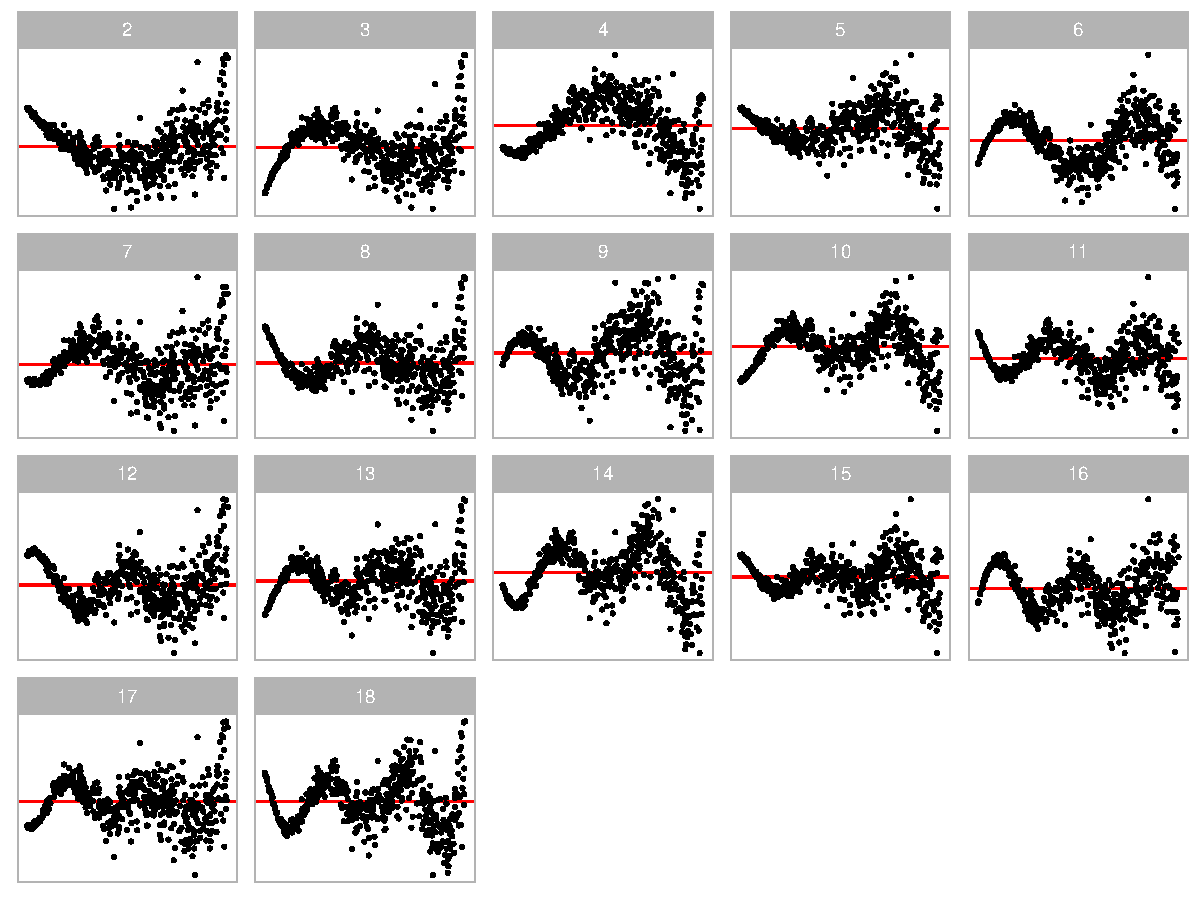
\includegraphics[width=1\linewidth]{paper_files/figure-latex/different-j-heter-1} 

}

\caption{Residual plots of models violating both the non-linearity and the heteroskedasticity assumptions. The 17 shapes are generated by varying the order of polynomial given by $j$ in $He_j(.)$, and the "left-triangle" shape is introduced by setting $a = -1$.}\label{fig:different-j-heter}
\end{figure}

\begin{figure}[!h]

{\centering 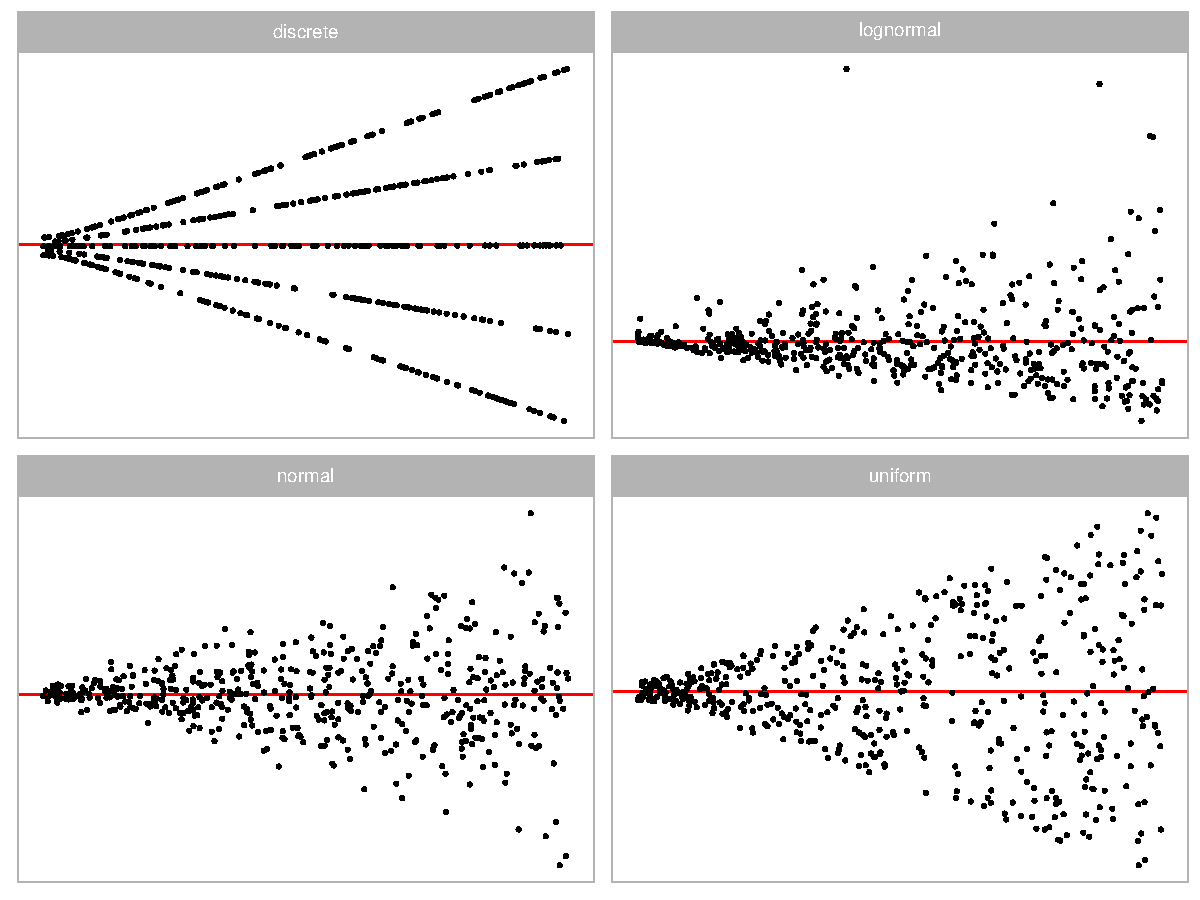
\includegraphics[width=1\linewidth]{paper_files/figure-latex/different-e-heter-1} 

}

\caption{Residual plots of models violating both the non-normality and the heteroskedasticity assumptions. The four shapes are generated by using four different error distributions including discrete, lognormal, normal and uniform, and the "left-triangle" shape is introduced by setting $a = -1$. }\label{fig:different-e-heter}
\end{figure}

Equation \ref{eq:data-sim} accommodates the incorporation of the second
predictor \(\boldsymbol{x}_2\). Introducing it into the data generation
process by setting \(\beta_1 = 1\) significantly enhances the complexity
of the shapes, as illustrated in Figure \ref{fig:different-j-x2}. In
comparison to Figure \ref{fig:different-j}, Figure
\ref{fig:different-j-x2} demonstrates that the non-linear shape
resembles a surface rather than a single curve. This augmentation can
facilitate the computer vision model in learning visual patterns from
residual plots of the multiple linear regression model.

In real-world analysis, it's not uncommon to encounter instances where
multiple model violations coexist. In such cases, the residual plots
often exhibit a mixed pattern of visual anomalies corresponding to
different types of model violations. Figure \ref{fig:different-j-heter}
and \ref{fig:different-e-heter} show the visual patterns of models with
multiple model violations.

\hypertarget{computation-of-scagnostics}{%
\subsubsection{Computation of
scagnostics}\label{computation-of-scagnostics}}

In Section \ref{introduction}, we mentioned that scagnostics consist of
a set of manually designed visual feature extraction functions. While
our computer vision model will learn its own feature extraction function
during training, leveraging additional information from scagnostics can
enhance the model's predictive accuracy.

For each generated residual plot, we computed four scagnostics --
``Monotonic,'' ``Sparse,'' ``Splines,'' and ``Striped'' -- using the
\texttt{cassowaryr} R package \citep{mason2022cassowaryr}. These
computed measures, along with the number of observations from the fitted
model, were provided as the second input for the computer vision model.
Although other scagnostics are informative, they are currently
unavailable due to a fatal bug in the compiled C program of the
\texttt{interp} R package \citep{Albrecht2023interp}, which may
unpredictably crash the process. For reproducibility, we excluded these
scagnostics from the training data.

\hypertarget{crafting-a-balanced-training-set}{%
\subsubsection{Crafting a balanced training
set}\label{crafting-a-balanced-training-set}}

To train a robust computer vision model, we deliberately controlled the
distribution of the target variable \(D\) in the training data. We
ensured that it followed a uniform distribution between \(0\) and \(7\).
This was achieved by organizing \(50\) buckets, each exclusively
accepting training samples with \(D\) falling within the range
\([7(i - 1)/49, 7i/49)\) for \(i < 50\), where \(i\) represents the
index of the \(i\)-th bucket. For the \(50\)-th bucket, any training
samples with \(D \geq 7\) were accepted.

With 80000 training images prepared, each bucket accommodated a maximum
of \(80000 \div 50 = 1600\) training samples. The simulator iteratively
sampled parameter values from the parameter space, generated residuals
and fitted values using the data generation process, computed the
distance, and checked if the sample fitted within the corresponding
bucket. This process continued until all buckets were filled.

Similarly, we adopted the same methodology to prepare 8000 test images
for performance evaluation and model diagnostics.

\hypertarget{architecture-of-the-computer-vision-model}{%
\subsection{Architecture of the computer vision
model}\label{architecture-of-the-computer-vision-model}}

The architecture of the computer vision model is adapted from a
well-established architecture known as VGG16, which has demonstrated
high performance in image classification \citep{simonyan2014very}.

The model begins with an input layer of shape
\(n \times h \times w \times 3\), capable of handling \(n\) RGB images.
This is followed by a grayscale conversion layer utilizing the luma
formula under the Rec. 601 standard, which converts the colour image to
grayscale. Grayscale suffices for our task since data points are plotted
in black. We experiment with three combinations of \(h\) and \(w\):
\(32 \times 32\), \(64 \times 64\), and \(128 \times 128\), aiming to
achieve sufficiently high image resolution for the problem at hand.

The processed image is used as the input for the first convolutional
block. The model comprises at most five consecutive convolutional
blocks, mirroring the original VGG16 architecture. Within each block,
there are two 2D convolutional layers followed by two activation layers,
respectively. Subsequently, a 2D max-pooling layer follows the second
activation layer. The 2D convolutional layer convolves the input with a
fixed number of \(3 \times 3\) convolution filters, while the 2D
max-pooling layer downsamples the input along its spatial dimensions by
taking the maximum value over a \(2 \times 2\) window for each channel
of the input. The activation layer employs the rectified linear unit
(ReLU) activation function, a standard practice in deep learning, which
introduces a non-linear transformation of the output of the 2D
convolutional layer. Additionally, to regularize training, a batch
normalization layer is added after each 2D convolutional layer and
before the activation layer. Finally, a dropout layer is appended at the
end of each convolutional block to randomly set some inputs to zero
during training, further aiding in regularization.

The output of the last convolutional block is summarized by either a
global max pooling layer or a global average pooling layer, resulting in
a two-dimensional tensor. To leverage the information contained in
scagnostics, this tensor is concatenated with an additional
\(n \times 5\) tensor, which contains the ``Monotonic,'' ``Sparse,''
``Splines,'' and ``Striped'' measures, along with the number of
observations for \(n\) residual plots.

The concatenated tensor is then fed into the final prediction block.
This block consists of two fully-connected layers. The first layer
contains at least \(128\) units, followed by a dropout layer.
Occasionally, a batch normalization layer is inserted between the
fully-connected layer and the dropout layer for regularization purposes.
The second fully-connected layer consists of only one unit, serving as
the output of the model.

The model weights \(\boldsymbol{\theta}\) were randomly initialized and
they were optimized by the Adam optimizer with the mean square error
loss function

\[\hat{\boldsymbol{\theta}} = \underset{\boldsymbol{\theta}}{argmin}\frac{1}{n_{train}}\sum_{i=1}^{n_{train}}(D_i - f_{\boldsymbol{\theta}}(V_i, S_i))^2,\]

\noindent where \(n_{train}\) is the number of training samples, \(V_i\)
is the \(i\)-th residual plot and \(S_i\) is the additional information
about the \(i\)-th residual plot including four scagnostics and the
number of observations.

\hypertarget{training-and-hyperparameter-tuning}{%
\subsection{Training and hyperparameter
tuning}\label{training-and-hyperparameter-tuning}}

To achieve an optimal deep learning model, hyperparameters like the
learning rate often need to be fine-tuned using a tuner. In our study,
we utilized the Bayesian optimization tuner from the \texttt{KerasTuner}
Python library \citep{omalley2019kerastuner} for this purpose. A
comprehensive list of hyperparameters is provided in Table
\ref{tab:hyperparameter}.

The ``number of base filters'' determines the number of filters for the
first 2D convolutional layer. In the VGG16 architecture, the number of
filters for the 2D convolutional layer in a block is typically twice the
number in the previous block, except for the last block, which maintains
the same number of convolution filters as the previous one. This
hyperparameter aids in controlling the complexity of the computer vision
model. Higher numbers of base filters result in more trainable
parameters. Likewise, the ``number of units for the fully-connected
layer'' determines the complexity of the final prediction block.
Increasing the number of units enhances model complexity, resulting in
more trainable parameters.

The dropout rate and batch normalization are flexible hyperparameters
that work in conjunction with other parameters to facilitate smooth
training. A higher dropout rate is necessary when the model tends to
overfit the training dataset by learning too much noise. Conversely, a
lower dropout rate is preferred when the model is complex and
challenging to converge. Batch normalization, on the other hand,
addresses the internal covariate shift problem arising from the
randomness in weight initialization and input data. It helps stabilize
and accelerate the training process by normalizing the activations of
each layer.

Additionally, incorporating additional inputs such as scagnostics and
the number of observations can potentially enhance prediction accuracy.
Therefore, we allowed the tuner to determine whether these inputs were
necessary for optimal model performance.

The learning rate is a crucial hyperparameter, as it dictates the step
size of the optimization algorithm. A high learning rate can help the
model avoid local minima but risks overshooting and missing the global
minimum. Conversely, a low learning rate smoothens the training process
but makes the convergence time longer and increases the likelihood of
getting trapped in local minima.

Our model was trained on the M3 high-performance computing platform,
using TensorFlow and Keras. During training, 80\% of the training data
was utilized for actual training, while the remaining 20\% was used as
validation data. The Bayesian optimization tuner conducted 100 trials to
identify the best hyperparameter values based on validation root mean
square error. The tuner then restored the best epoch of the best model
from the trials. Additionally, we applied early stopping, terminating
the training process if the validation root mean square error fails to
improve for 50 epochs. The maximum allowed epochs was set at 2000,
although no models reached this threshold.

\begin{table}

\caption{\label{tab:hyperparameter}Name of hyperparameters and their correspoding domain for the computer vision model.}
\centering
\begin{tabular}[t]{ll}
\toprule
Hyperparameter & Domain\\
\midrule
Number of base filters & \{4, 8, 16, 32, 64\}\\
Dropout rate for convolutional blocks & {}[0.1, 0.6]\\
Batch normalization for convolutional blocks & \{false, true\}\\
Type of global pooling & \{max, average\}\\
Ignore additional inputs & \{false, true\}\\
\addlinespace
Number of units for the fully-connected layer & \{128, 256, 512, 1024, 2048\}\\
Batch normalization for the fully-connected layer & \{false, true\}\\
Dropout rate for the fully-connected layer & {}[0.1, 0.6]\\
Learning rate & {}[1e-8, 1e-1]\\
\bottomrule
\end{tabular}
\end{table}

\hypertarget{model-evaluation-methods}{%
\subsection{Model evaluation methods}\label{model-evaluation-methods}}

This section remains incomplete as we may modify the ``Results'' section
later on.

\hypertarget{results}{%
\section{Results}\label{results}}

\hypertarget{optimized-hyperparameters}{%
\subsection{Optimized hyperparameters}\label{optimized-hyperparameters}}

Based on the tuning process described in Section
\ref{training-and-hyperparameter-tuning}, the optimized hyperparameter
values are presented in Table \ref{tab:best-hyperparameter}. It was
observable that a minimum of \(32\) base filters was necessary, with the
preferable choice being \(64\) base filters for both the
\(64 \times 64\) and \(128 \times 128\) models, mirroring the original
VGG16 architecture. The optimized dropout rate for convolutional blocks
hovered around \(0.4\), and incorporating batch normalization for
convolutional blocks proved beneficial for performance.

All optimized models chose to retain the additional inputs, contributing
to the reduction of validation error. The number of units required for
the fully-connected layer was \(256\), a relatively modest number
compared to the VGG16 classifier, suggesting that the problem at hand
was relatively straightforward. The optimized learning rates were
typically smaller than the default value recommended by Keras, which is
0.001.

\begin{table}

\caption{\label{tab:best-hyperparameter}Hyperparameters values for the optimized computer vision models with different input sizes.}
\centering
\resizebox{\linewidth}{!}{
\begin{tabular}[t]{llll}
\toprule
Hyperparameter & $32 \times 32$ & $64 \times 64$ & $128 \times 128$\\
\midrule
Number of base filters & 32 & 64 & 64\\
Dropout rate for convolutional blocks & 0.4 & 0.3 & 0.4\\
Batch normalization for convolutional blocks & true & true & true\\
Type of global pooling & max & average & average\\
Ignore additional inputs & false & false & false\\
\addlinespace
Number of units for the fully-connected layer & 256 & 256 & 256\\
Batch normalization for the fully-connected layer & false & true & true\\
Dropout rate for the fully-connected layer & 0.2 & 0.4 & 0.1\\
Learning rate & 0.0003 & 0.0006 & 0.0052\\
\bottomrule
\end{tabular}}
\end{table}

\hypertarget{model-performance}{%
\subsection{Model performance}\label{model-performance}}

The training and test performance for the optimized models with three
different input sizes are summarized in Table \ref{tab:performance}.
Among these models, the \(64 \times 64\) model and the \(32 \times 32\)
model consistently exhibited the best training and test performance,
respectively. The mean absolute error indicated that the difference
between \(\hat{D}\) and \(D\) was approximately \(0.43\) on the test
set, a negligible deviation considering the normal range of \(D\)
typically falls between \(0\) and \(7\). The high \(R^2\) values also
suggested that the predictions were largely linearly correlated with the
target.

Figure \ref{fig:model-performance} presents a hexagonal heatmap for
\(D - \hat{D}\) versus \(\hat{D}\). The red smoothing curves, fitted by
generalized additive models \citep{hastie2017generalized}, demonstrate
that all the optimized models perform admirably on both the training and
test sets. No structural issues are noticeable in Figure
\ref{fig:model-performance}, but some minor issues regarding
over-prediction and under-prediction are observed.

The figure highlights that most under-predictions occurred when
\(\hat{D} < 3\), while over-predictions occurred predominantly when
\(3 < \hat{D} < 6\). To comprehend the reasons behind these deviations,
we fitted a regression tree using the \texttt{rpart} R package
\citep{Terry2022rpart} on \(D - \hat{D}\) for all factors used in the
data generating process. The results of the regression tree are provided
in the Appendix.

The regression tree revealed that most issues arose from non-linearity
problems and the presence of a second predictor in the regression model.
When the error distribution had a very small variance, all computer
vision models tended to under-predict the distance. Conversely, when the
error distribution had a large variance, all models tended to
over-predict the distance. Therefore, Additionally, for input images
representing null plots, it was expected that the models will
over-predict the distance, as explained in Section
\ref{null-distribution-of-the-approximated-distance}.

Since most of the deviation stemmed from the presence of non-linearity
violations, to further investigate this, we split the test set and
re-evaluated the performance, as detailed in Table
\ref{tab:performance-sub}. It was evident that metrics for null plots
were notably worse compared to other categories. Furthermore, residual
plots solely exhibiting non-normality issues were the easiest to
predict, with very low test root mean square error (RMSE) around
\(0.3\), very low mean absolute error (MAE) around \(0.2\), and very
high \(R^2\) around \(0.94\). Residual plots with non-linearity issues
were more challenging to assess than those with heteroskedasticity or
non-normality issues. Assessing residual plots with heteroskedasticity
was not as difficult as assessing those with non-linearity issues. When
multiple violations were introduced to a residual plot, the performance
metrics typically lay between the metrics for each individual violation.

Based on the model performance metrics, we will only use the
best-performing model evaluated on the test set, namely the
\(32 \times 32\) model, for the subsequent analysis.

\begin{table}

\caption{\label{tab:performance}The training and test performance of three optimized models with different input sizes. The best metrics are colored in red.}
\centering
\begin{tabular}[t]{l>{}l>{}l>{}l>{}l}
\toprule
 & RMSE & $R^2$ & MAE & Huber loss\\
\midrule
\addlinespace[0.3em]
\multicolumn{5}{l}{\textbf{Training set}}\\
\hspace{1em}$32 \times 32$ & \textcolor{black}{0.531} & \textcolor{black}{0.937} & \textcolor{black}{0.364} & \textcolor{black}{0.126}\\
\hspace{1em}$64 \times 64$ & \textcolor{red}{0.405} & \textcolor{red}{0.963} & \textcolor{red}{0.260} & \textcolor{red}{0.072}\\
\hspace{1em}$128 \times 128$ & \textcolor{black}{0.432} & \textcolor{black}{0.959} & \textcolor{black}{0.290} & \textcolor{black}{0.084}\\
\addlinespace[0.3em]
\multicolumn{5}{l}{\textbf{Test set}}\\
\hspace{1em}$32 \times 32$ & \textcolor{red}{0.660} & \textcolor{red}{0.901} & \textcolor{red}{0.434} & \textcolor{red}{0.181}\\
\hspace{1em}$64 \times 64$ & \textcolor{black}{0.674} & \textcolor{black}{0.897} & \textcolor{black}{0.438} & \textcolor{black}{0.186}\\
\hspace{1em}$128 \times 128$ & \textcolor{black}{0.692} & \textcolor{black}{0.892} & \textcolor{black}{0.460} & \textcolor{black}{0.199}\\
\bottomrule
\end{tabular}
\end{table}

\begin{figure}[!h]

{\centering 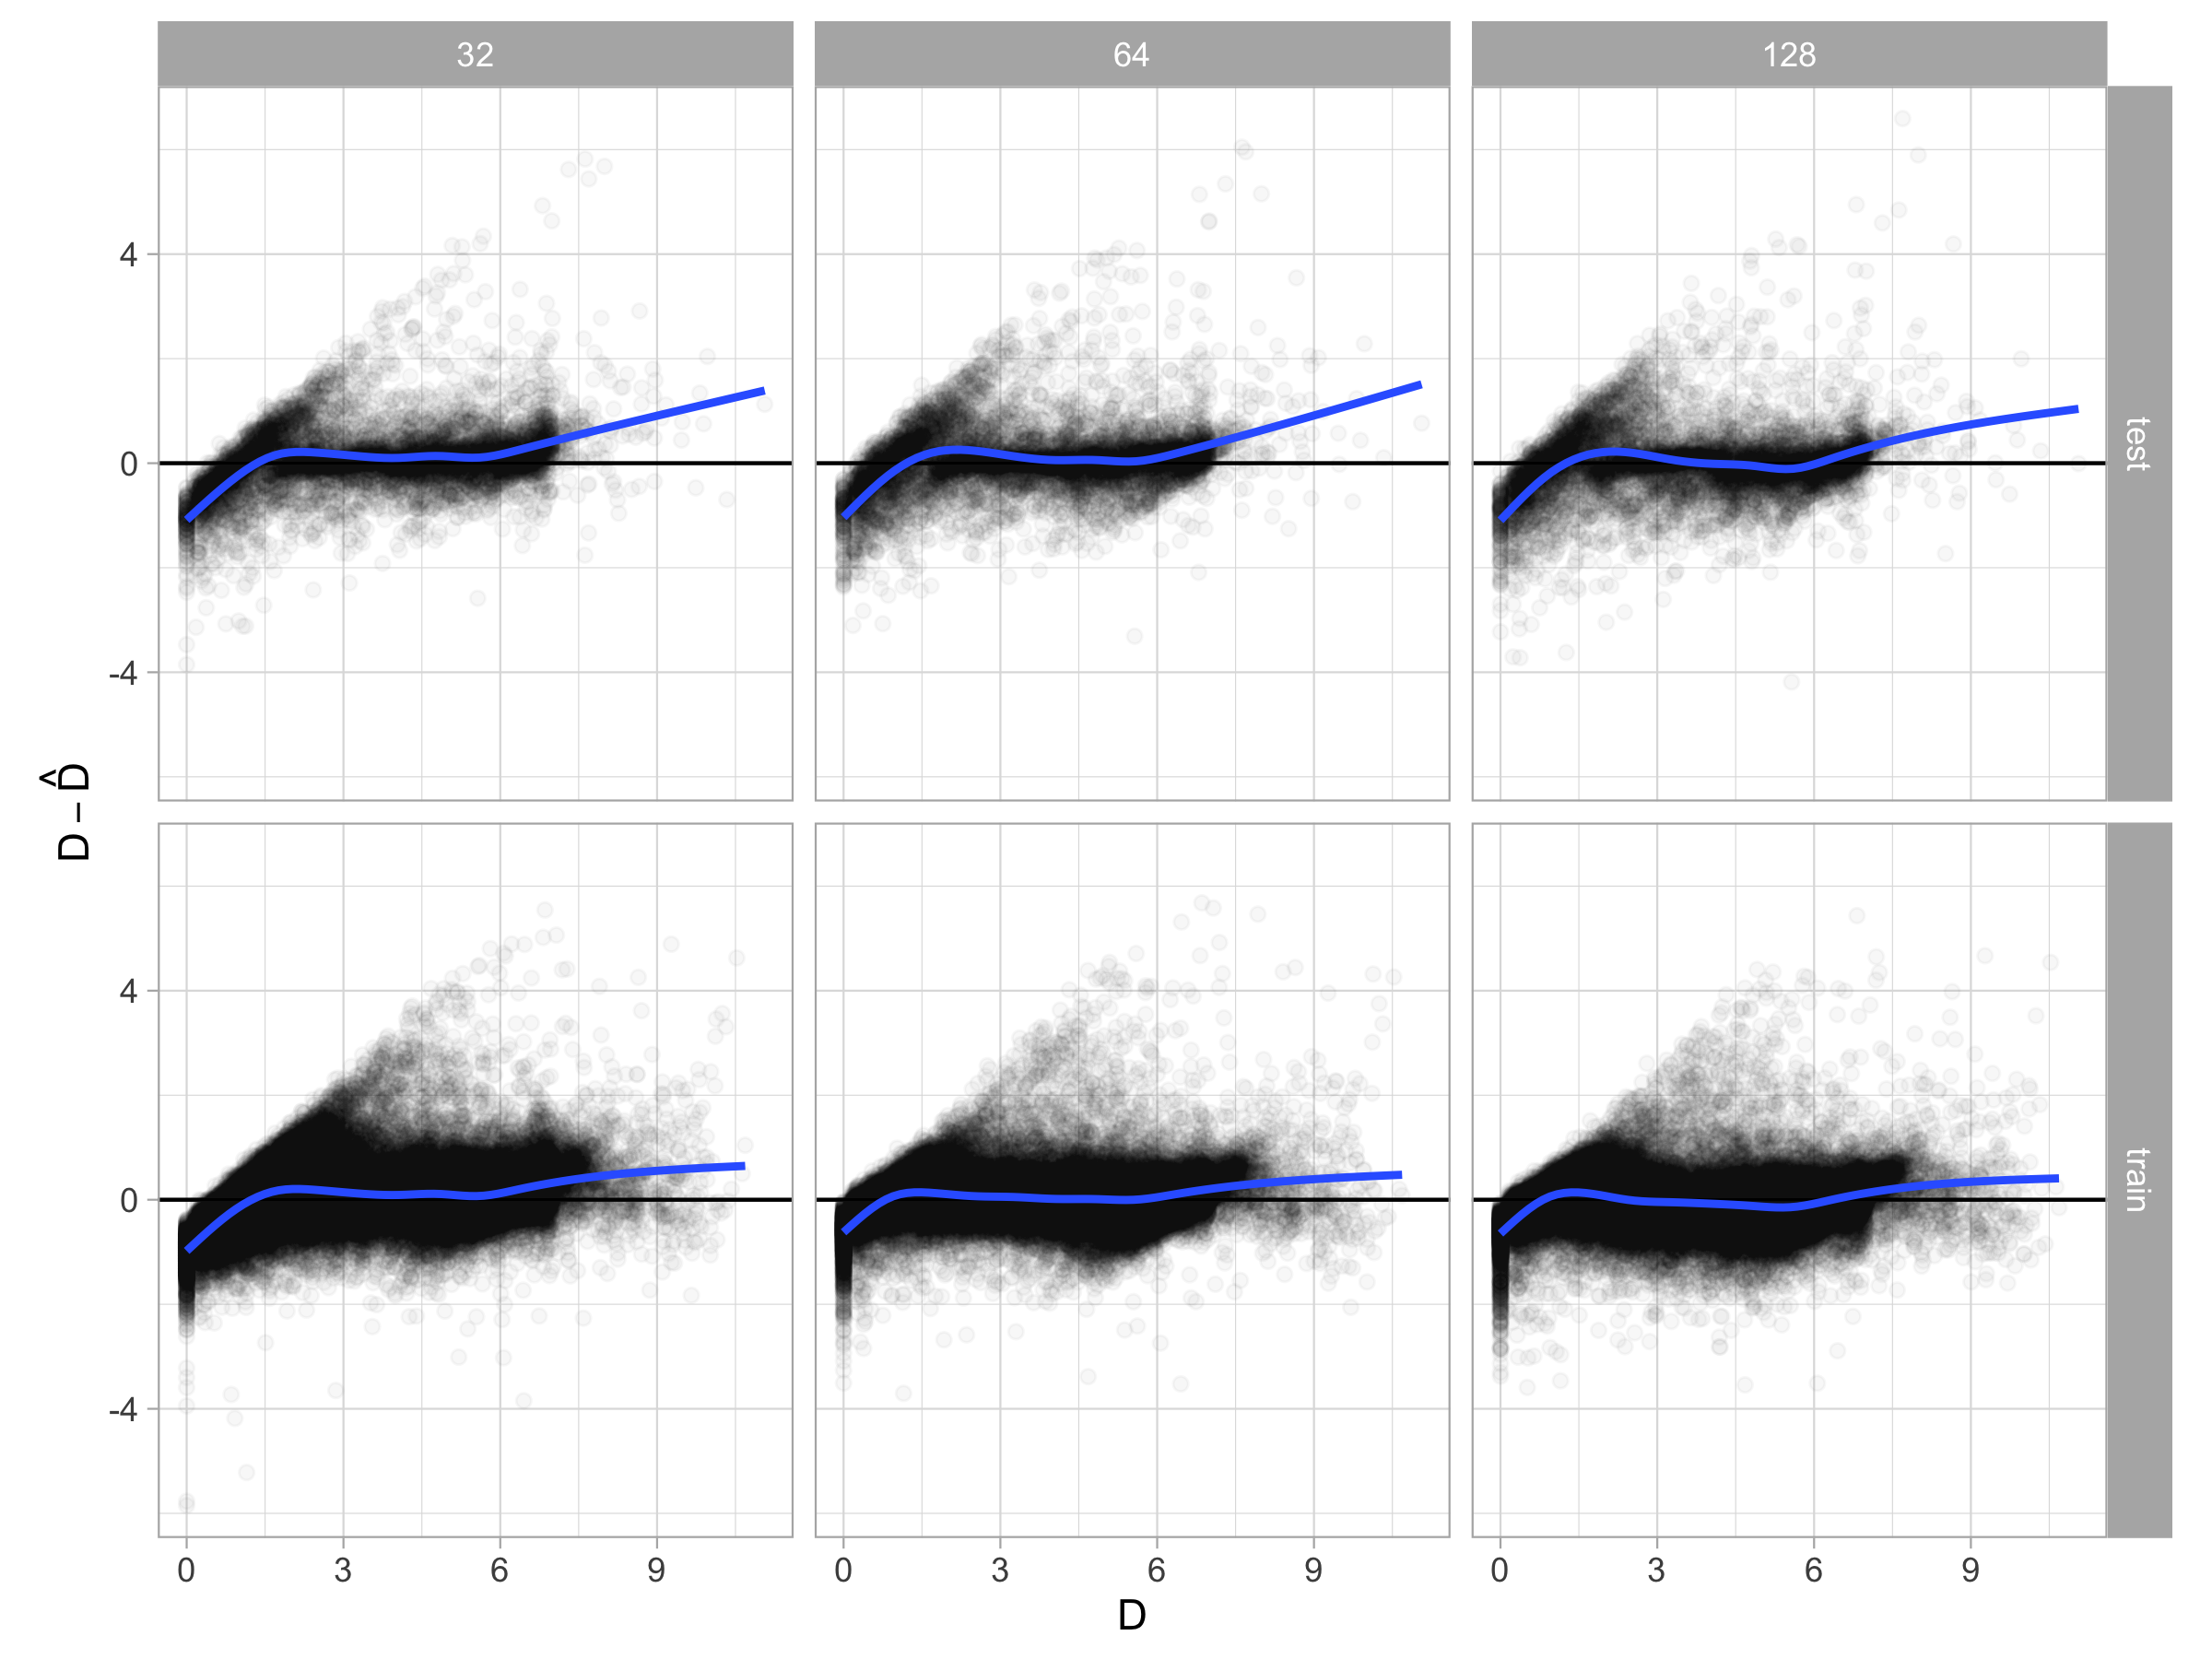
\includegraphics[width=1\linewidth]{paper_files/figure-latex/model-performance-1} 

}

\caption{Hexagonal heatmap for residuals vs predicted distance on training and test data for three optimized models with different input sizes. The red lines are smoothing curves produced by fitting gnealized additive models. The area over the zero line in light pink indicates under-prediction, and the area under the zero line in light green indicates over-prediction.}\label{fig:model-performance}
\end{figure}

\begin{table}

\caption{\label{tab:performance-sub}The training and test performance of the $32 \times 32$ model presented with different model violations.  The best metrics are colored in red.}
\centering
\resizebox{\linewidth}{!}{
\begin{tabular}[t]{ll>{}l>{}l>{}l>{}l}
\toprule
Violations & \#samples & RMSE & $R^2$ & MAE & Huber loss\\
\midrule
\addlinespace[0.3em]
\multicolumn{6}{l}{\textbf{Training set}}\\
\hspace{1em}no violations & 1546 & \textcolor{black}{1.149} & \textcolor{black}{} & \textcolor{black}{1.080} & \textcolor{black}{0.592}\\
\hspace{1em}non-linearity & 22184 & \textcolor{black}{0.625} & \textcolor{black}{0.851} & \textcolor{black}{0.474} & \textcolor{black}{0.177}\\
\hspace{1em}heteroskedasticity & 10826 & \textcolor{black}{0.528} & \textcolor{black}{0.942} & \textcolor{black}{0.407} & \textcolor{black}{0.133}\\
\hspace{1em}non-linearity + heteroskedasticity & 10221 & \textcolor{black}{0.593} & \textcolor{black}{0.920} & \textcolor{black}{0.439} & \textcolor{black}{0.158}\\
\hspace{1em}non-normality & 10797 & \textcolor{red}{0.279} & \textcolor{red}{0.955} & \textcolor{red}{0.177} & \textcolor{red}{0.038}\\
\hspace{1em}non-linearity + non-normality & 8835 & \textcolor{black}{0.472} & \textcolor{black}{0.923} & \textcolor{black}{0.274} & \textcolor{black}{0.090}\\
\hspace{1em}heteroskedasticity + non-normality & 7870 & \textcolor{black}{0.354} & \textcolor{black}{0.905} & \textcolor{black}{0.211} & \textcolor{black}{0.052}\\
\hspace{1em}non-linearity + heteroskedasticity + non-normality & 7721 & \textcolor{black}{0.432} & \textcolor{black}{0.874} & \textcolor{black}{0.261} & \textcolor{black}{0.078}\\
\addlinespace[0.3em]
\multicolumn{6}{l}{\textbf{Test set}}\\
\hspace{1em}no violations & 155 & \textcolor{black}{1.267} & \textcolor{black}{} & \textcolor{black}{1.174} & \textcolor{black}{0.685}\\
\hspace{1em}non-linearity & 2218 & \textcolor{black}{0.787} & \textcolor{black}{0.771} & \textcolor{black}{0.578} & \textcolor{black}{0.257}\\
\hspace{1em}heteroskedasticity & 1067 & \textcolor{black}{0.602} & \textcolor{black}{0.922} & \textcolor{black}{0.461} & \textcolor{black}{0.170}\\
\hspace{1em}non-linearity + heteroskedasticity & 985 & \textcolor{black}{0.751} & \textcolor{black}{0.868} & \textcolor{black}{0.541} & \textcolor{black}{0.236}\\
\hspace{1em}non-normality & 1111 & \textcolor{red}{0.320} & \textcolor{red}{0.942} & \textcolor{red}{0.194} & \textcolor{red}{0.049}\\
\hspace{1em}non-linearity + non-normality & 928 & \textcolor{black}{0.600} & \textcolor{black}{0.879} & \textcolor{black}{0.335} & \textcolor{black}{0.133}\\
\hspace{1em}heteroskedasticity + non-normality & 819 & \textcolor{black}{0.489} & \textcolor{black}{0.832} & \textcolor{black}{0.267} & \textcolor{black}{0.093}\\
\hspace{1em}non-linearity + heteroskedasticity + non-normality & 717 & \textcolor{black}{0.620} & \textcolor{black}{0.762} & \textcolor{black}{0.339} & \textcolor{black}{0.140}\\
\bottomrule
\end{tabular}}
\end{table}

\hypertarget{model-violations-index-mvi}{%
\subsection{Model Violations Index
(MVI)}\label{model-violations-index-mvi}}

Figures \ref{fig:poly-index} and \ref{fig:heter-index} display the
residual plots for fitted models exhibiting varying degrees of
non-linearity and heteroskedasticity. Each residual plot's Model
Violation Index (MVI) is computed using Equation \ref{eq:mvi} with
\(C = 10\). When \(\text{MVI} > 8\), the visual patterns are notably
strong and easily discernible by humans. In the range
\(6 < \text{MVI} < 8\), the visibility of the visual pattern diminishes
as MVI decreases. Conversely, when \(\text{MVI} < 6\), the visual
pattern tends to become relatively faint and challenging to observe.
Table \ref{tab:mvi} provides a summary of the MVI usage and it is
applicable to other linear regression models.

\begin{table}

\caption{\label{tab:mvi}Degree of model violations or the strength of the visual signals according to the Model Violation Index (MVI). The constant $C$ is set to be 10.}
\centering
\begin{tabular}[t]{ll}
\toprule
Degree of model violations & Range ($C$ = 10)\\
\midrule
Strong & $\text{MVI} > 8$\\
Moderate & $6 < \text{MVI} < 8$\\
Weak & $\text{MVI} < 6$\\
\bottomrule
\end{tabular}
\end{table}

\begin{figure}[!h]

{\centering 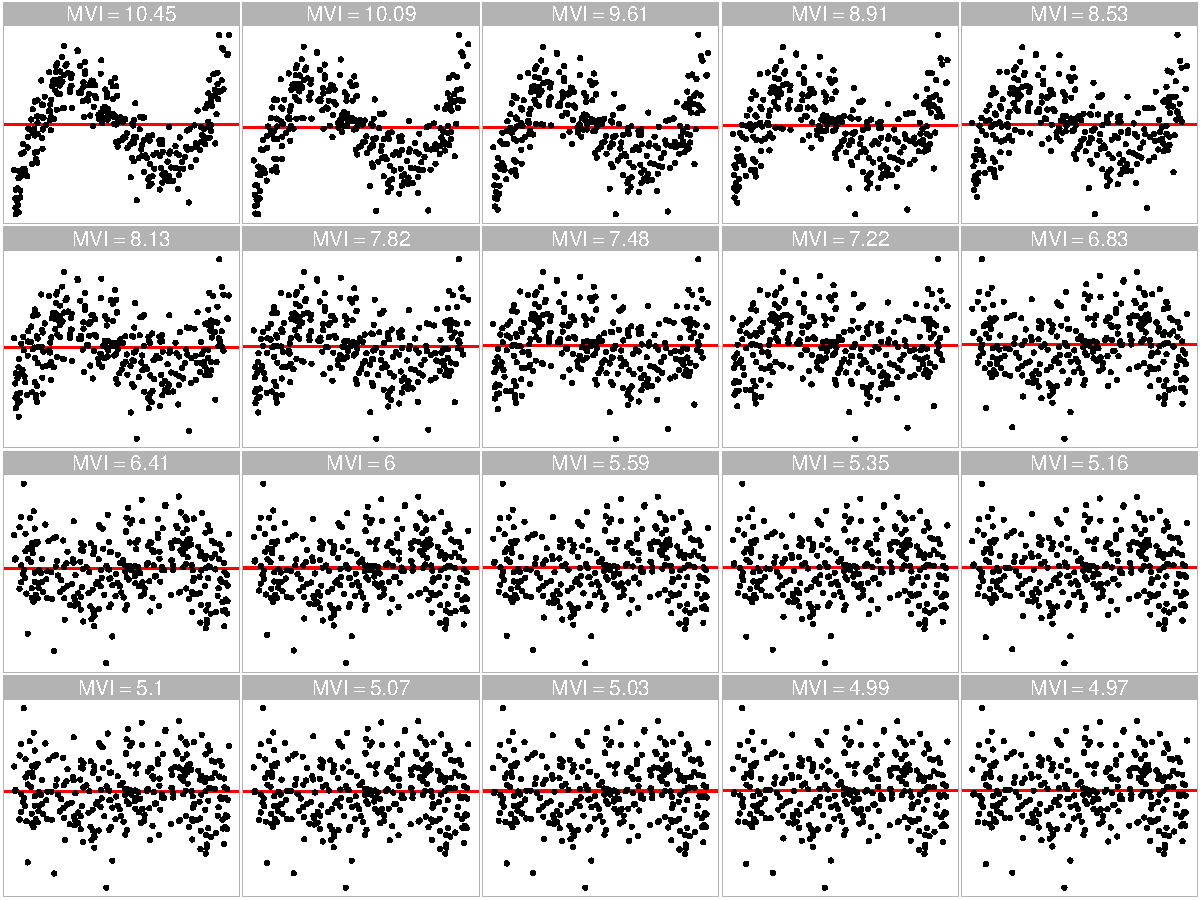
\includegraphics[width=1\linewidth]{paper_files/figure-latex/poly-index-1} 

}

\caption{Residual plots generated from fitted models exhibiting varying degrees of non-linearity violations. The Model violations index (MVI) is displayed atop each residual plot. The non-linearity patterns are relatively strong for $MVI > 8$, and relatively weak for $MVI < 6$.}\label{fig:poly-index}
\end{figure}

\begin{figure}[!h]

{\centering 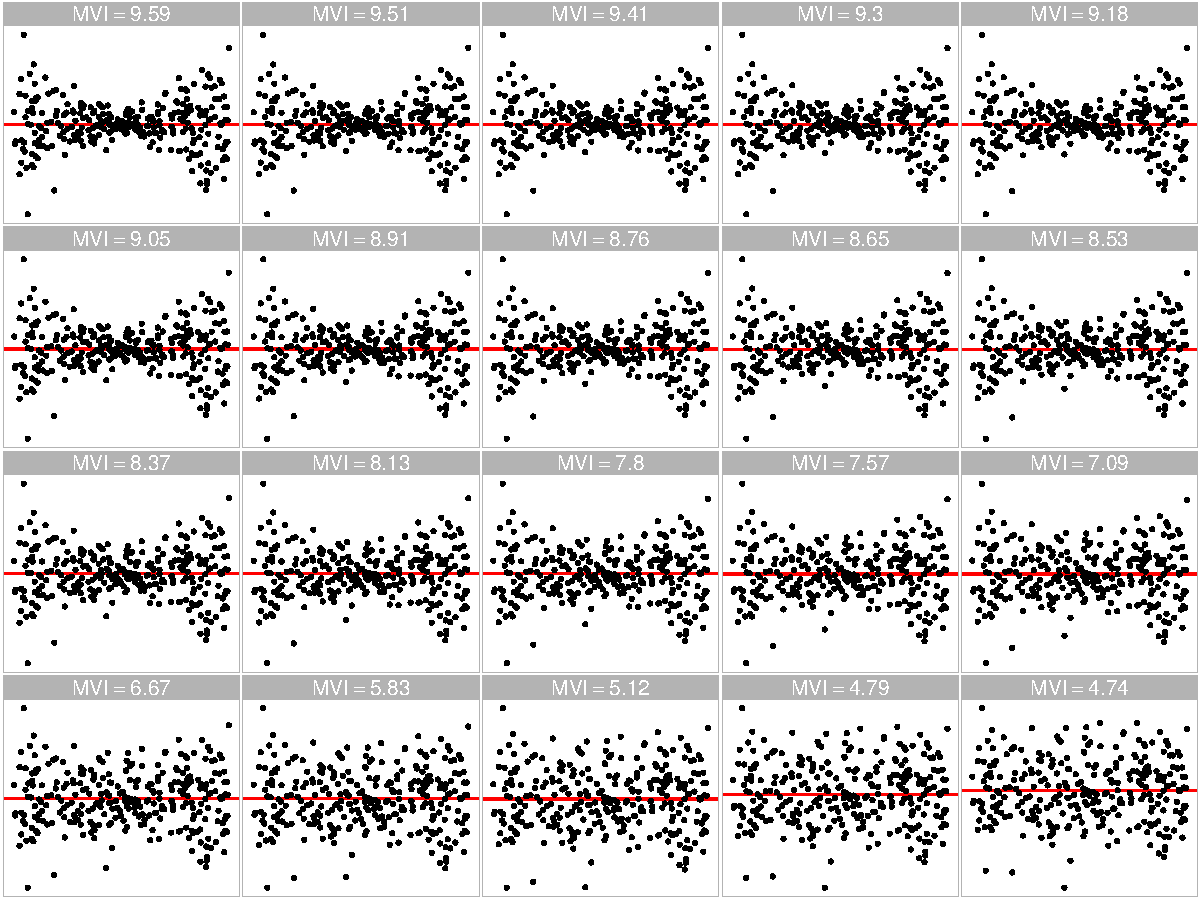
\includegraphics[width=1\linewidth]{paper_files/figure-latex/heter-index-1} 

}

\caption{Residual plots generated from fitted models exhibiting varying degrees of heteroskedasticity violations. The Model violations index (MVI) is displayed atop each residual plot. The heteroskedasticity patterns are relatively strong for $MVI > 8$, and relatively weak for $MVI < 6$.}\label{fig:heter-index}
\end{figure}

\hypertarget{comparison-with-human-visual-inference-and-conventional-tests}{%
\subsection{Comparison with human visual inference and conventional
tests}\label{comparison-with-human-visual-inference-and-conventional-tests}}

\hypertarget{overview-of-the-human-subject-experiment}{%
\subsubsection{Overview of the human subject
experiment}\label{overview-of-the-human-subject-experiment}}

In order to check the validity of the proposed computer vision model,
residual plots presented in the human subject experiment conducted by
\citet{li2023plot} will be assessed. This study has collected \(7974\)
human responses to \(1152\) lineups. Each lineup contains one randomly
placed actual residual plot and 19 null plots. Among the \(1152\)
lineups, \(24\) are attention check lineups in which the visual patterns
are designed to be extremely obvious and very different from the
corresponding to null plots, \(36\) are null lineups where all the
lineups consist of only null plots, \(279\) are lineups with uniform
predictor distribution evaluated by \(11\) participants, and the
remaining \(813\) are lineups with discrete, skewed or normal predictor
distribution evaluated by \(5\) participants. Attention check lineups
and null lineups will not be assessed in the following analysis.

In \citet{li2023plot}, the residual plots are simulated from a data
generating process which is a special case of Equation
\ref{eq:data-sim}. The main characteristic is the model violations are
introduced separately, meaning non-linearity and heteroskedasticity will
not co-exist in one lineup but assigned uniformly to all lineups.
Additionally, non-normality and multiple predictors are not considered
in the experimental design.

\hypertarget{model-performance-on-the-human-data}{%
\subsubsection{Model performance on the human
data}\label{model-performance-on-the-human-data}}

\begin{table}

\caption{\label{tab:experiment-performance}The performance of the $32 \times 32$ model on the data used in the human subject experiment.}
\centering
\begin{tabular}[t]{lllll}
\toprule
Voilation & RMSE & $R^2$ & MAE & Huber loss\\
\midrule
heteroskedasticity & 0.721 & 0.852 & 0.553 & 0.235\\
non-linearity & 0.738 & 0.770 & 0.566 & 0.246\\
\bottomrule
\end{tabular}
\end{table}

For each lineup used in \citet{li2023plot}, there is one actual residual
plot and 19 null plots. While the distance \(D\) for the actual residual
plot depends on the underlying data generating process, the distance
\(D\) for the null plots is zero. We have used our optimized computer
vision model to predict \(\hat{D}\) for both the actual residual plots
and the null plots. Additionally, the appropriate conventional tests
including the Ramsey Regression Equation Specification Error Test
(RESET) \citep{ramsey1969tests} for non-linearity and the Breusch-Pagan
test \citep{breusch1979simple} for heteroskedasticity were applied on
the same data for comparison.

The performance metrics of \(\hat{D}\) for actual residual plots are
outlined in Table \ref{tab:experiment-performance}. It's notable that
all performance metrics are slightly worse than those evaluated on the
test data. Nevertheless, the mean absolute error remains at a low level,
and the linear correlation between the prediction and the true value
remains very high. Lineups with non-linearity issues are more
challenging to predict than those with heteroskedasticity issues.

For null plots, a histogram of the predictions is provided in Figure
\ref{fig:hist-null-human}. In most cases, \(\hat{D}\) is predicted to be
around \(1\). As \(\hat{D}\) increases, the number of predictions
decreases. The 90\% and 95\% sample quantiles are approximately at
\(2\), and the 99\% sample quantile is around \(2.5\). These sample
quantiles can serve as global critical values for determining whether a
residual plot needs to be rejected. We have also computed the 95\%
sample quantiles by assessing 200 null plots for each fitted model used
in the experiment. The difference between decisions based on these two
types of critical values is minor, with decisions aligning 93.8\% of the
time. Therefore, we will be using the 95\% sample quantiles obtained
from each fitted model in the following analysis.

Likewise, Figure \ref{fig:conv-mosaic} and Table \ref{tab:conv-table}
provide a summary of the agreement between decisions made by the
computer vision model and conventional tests. The agreement rates
between conventional tests and the computer vision model are 65.37\% and
57.29\% for residual plots containing heteroskedasticity and
non-linearity patterns, respectively. These figures are lower than those
presented in Table \ref{tab:human-table}, indicating that the computer
vision model exhibits behaviour more akin to visual tests than
conventional tests. Additionally, conventional tests tend to reject
residual plots almost exclusively when the computer vision model does,
but they also reject plots when the computer vision model does not. This
suggests that conventional tests are more sensitive than the computer
vision model.

When plotting the decision against the distance, as illustrated in
Figure \ref{fig:power}, several observations emerge. Firstly, for the
computer vision model, when the distance \(D > 3\), almost all residual
plots are rejected. However, for visual tests conducted by humans, the
threshold is higher, set at \(D > 5\). And conventional tests exhibit
some non-rejection cases for \(D > 3\). Moreover, the computer vision
model tends to have fewer rejected cases than conventional tests when
\(D < 2\). However, visual tests demonstrate the lowest sensitivity to
residual plots with small distances. Therefore, tests based on the
computer vision model are less sensitive to small deviations from model
assumptions than conventional tests but more sensitive to moderate
deviations. Rejection decisions are fitted by logistic regression models
with no intercept terms but an offset equals to
\(\text{log}(0.05/0/95)\). The fitting curves for the computer vision
model fall between those of conventional tests and visual tests for
non-linearity and are slightly below conventional tests for
heteroskedasticity. There is still potential to refine the computer
vision model to better align its behaviour with visual tests.

Figure \ref{fig:delta} displays the scatter plot of the weighted
detection rate vs the \(\delta\)-difference. In the experiment conducted
in \citet{li2023plot}, participants were allowed to make multiple
selections for a lineup. The weighted detection rate is computed by
assigning weights to each detection. If the participant selects zero
plots, the corresponding weight is 0.05; otherwise, the weight is 1
divided by the number of selections. The \(\delta\)-difference is
defined by \citet{chowdhury2018measuring} as

\begin{equation}
\delta = \hat{D} - \underset{j}{max}\left(\hat{D}_{null}^{(j)}\right) \quad \text{for}~j = 1,...,m-1,
\end{equation}

\noindent where \(\hat{D}_{null}^{(j)}\) is the approximated distance
for the \(j\)-th null plot, and \(m\) is the number of plots in a
lineup.

Figure \ref{fig:delta} indicates that the weighted detection rate
increases as the \(\delta\)-difference increases, particularly when the
\(\delta\)-difference is greater than zero. A negative
\(\delta\)-difference suggests that there is at least one null plot in
the lineup with a stronger visual signal than the actual residual plot.
In some instances, the weighted detection rate is close to one, yet the
\(\delta\)-difference is negative. This discrepancy implies that the
distance measure, or the approximated distance, may not perfectly
reflect actual human behaviour.

\begin{figure}[!h]

{\centering 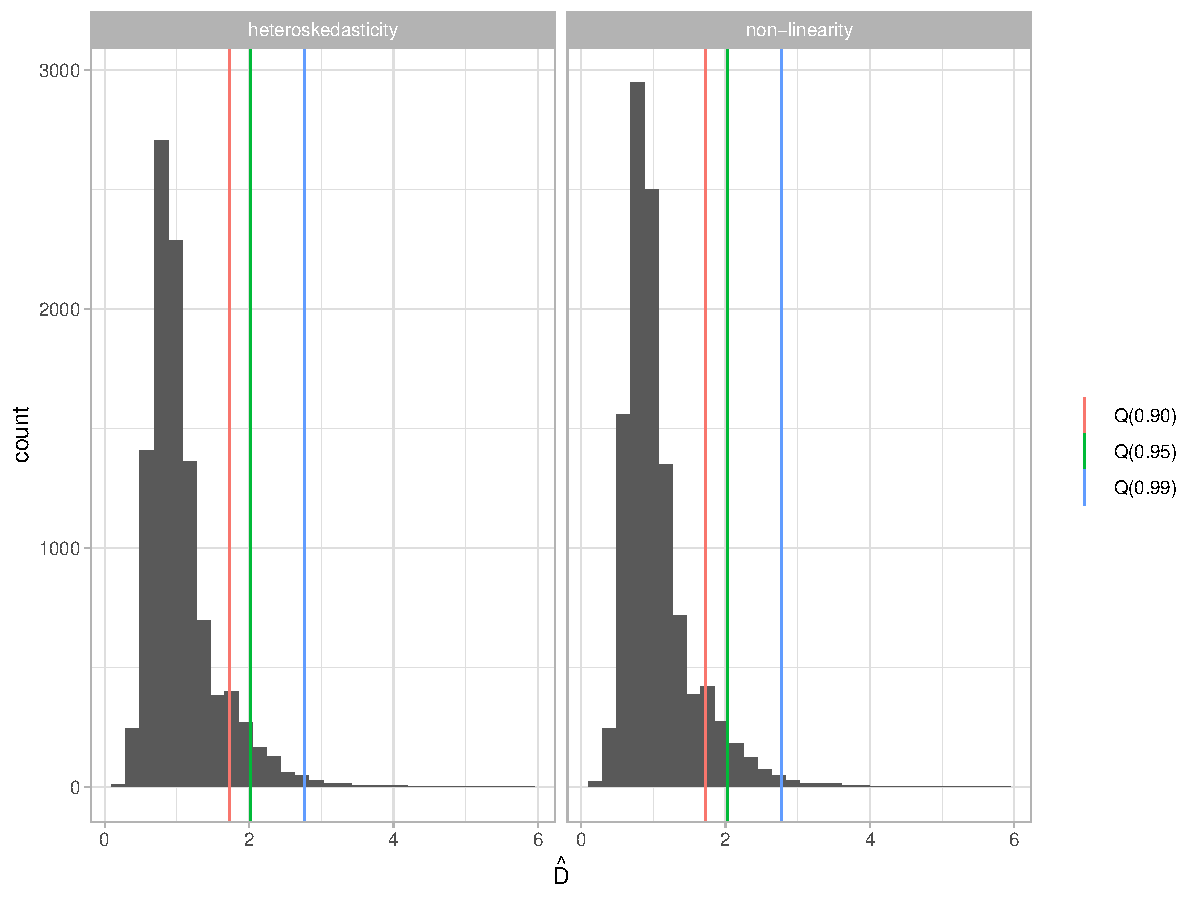
\includegraphics[width=1\linewidth]{paper_files/figure-latex/hist-null-human-1} 

}

\caption{Histogram of predicted distance on null plots used in the human subject experiment. Sample quantiles are drawn in different colors.}\label{fig:hist-null-human}
\end{figure}

\begin{table}

\caption{\label{tab:human-table}Summary of decisions made by visual tests conducted by human and decisions made by the computer vision model.}
\centering
\begin{tabular}[t]{llll}
\toprule
Violations & \#Samples & \#Agreements & Agreement rate\\
\midrule
heteroskedasticity & 540 & 367 & 0.6796\\
non-linearity & 576 & 385 & 0.6684\\
\bottomrule
\end{tabular}
\end{table}

\begin{table}

\caption{\label{tab:conv-table}Summary of decisions made by conventional tests and decisions made by the computer vision model.}
\centering
\begin{tabular}[t]{llll}
\toprule
Violations & \#Samples & \#Agreements & Agreement rate\\
\midrule
heteroskedasticity & 540 & 464 & 0.6537\\
non-linearity & 576 & 459 & 0.5729\\
\bottomrule
\end{tabular}
\end{table}

\begin{figure}[!h]

{\centering 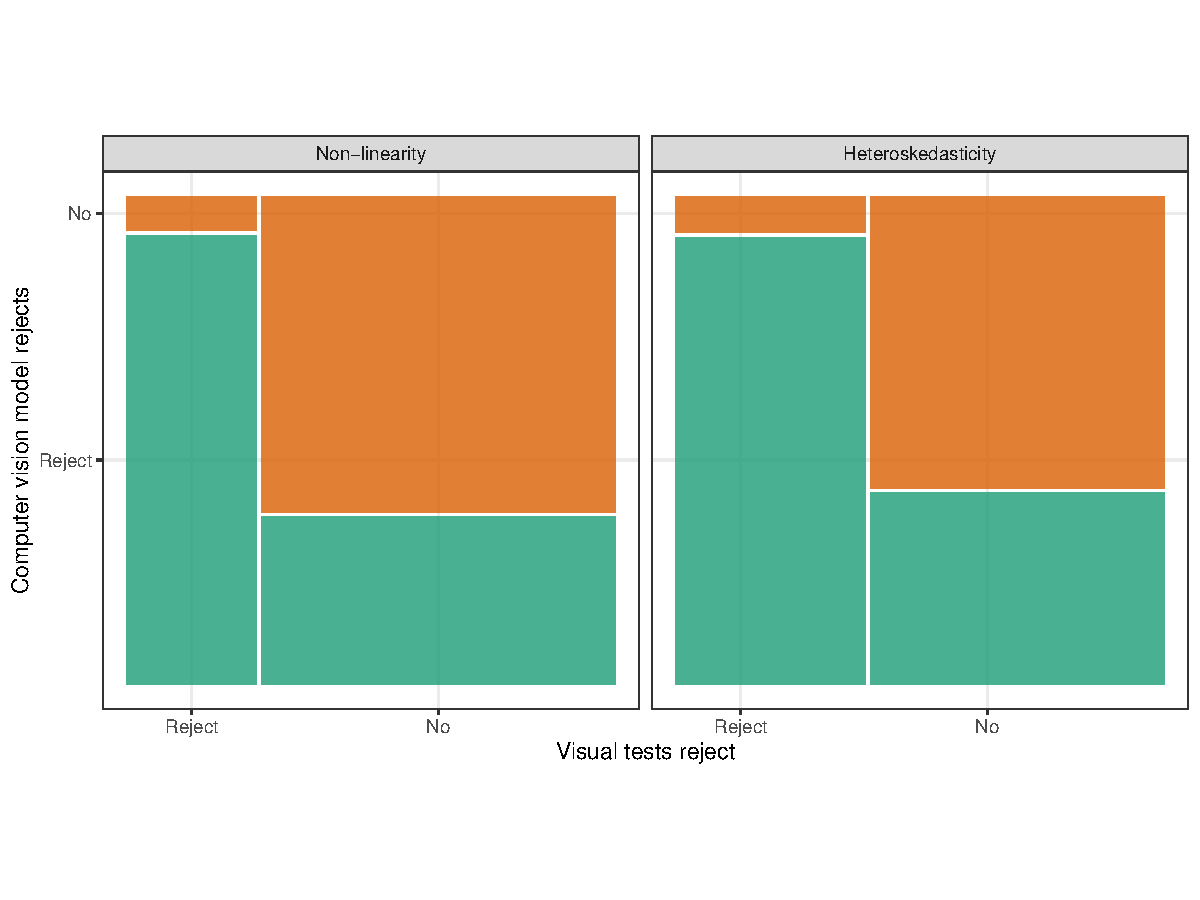
\includegraphics[width=1\linewidth]{paper_files/figure-latex/human-mosaic-1} 

}

\caption{Rejection rate ($p$-value $\leq0.05$) of visual test conditional on the computer vision model decision on non-linearity (left) and heteroskedasticity (right) lineups displayed using a mosaic plot. The visual test rejects less frequently than the computer vision model, and (almost) only rejects when the computer vision model does.}\label{fig:human-mosaic}
\end{figure}

\begin{figure}[!h]

{\centering 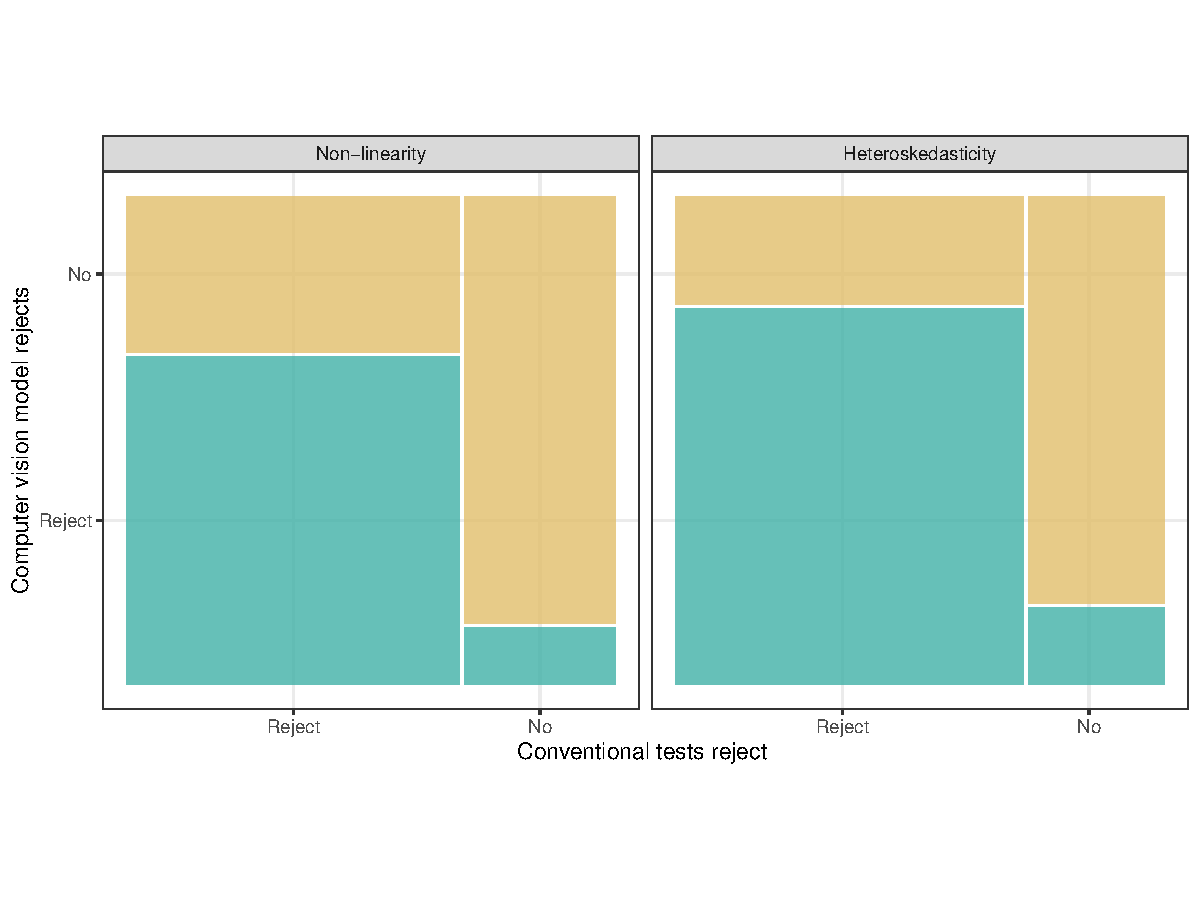
\includegraphics[width=1\linewidth]{paper_files/figure-latex/conv-mosaic-1} 

}

\caption{Rejection rate ($p$-value $\leq0.05$) of conventional test conditional on the computer vision model decision on non-linearity (left) and heteroskedasticity (right) lineups displayed using a mosaic plot. The conventional test rejects more frequently than the computer vision model, and (almost) only rejects when the computer vision model does.}\label{fig:conv-mosaic}
\end{figure}

\begin{figure}[!h]

{\centering 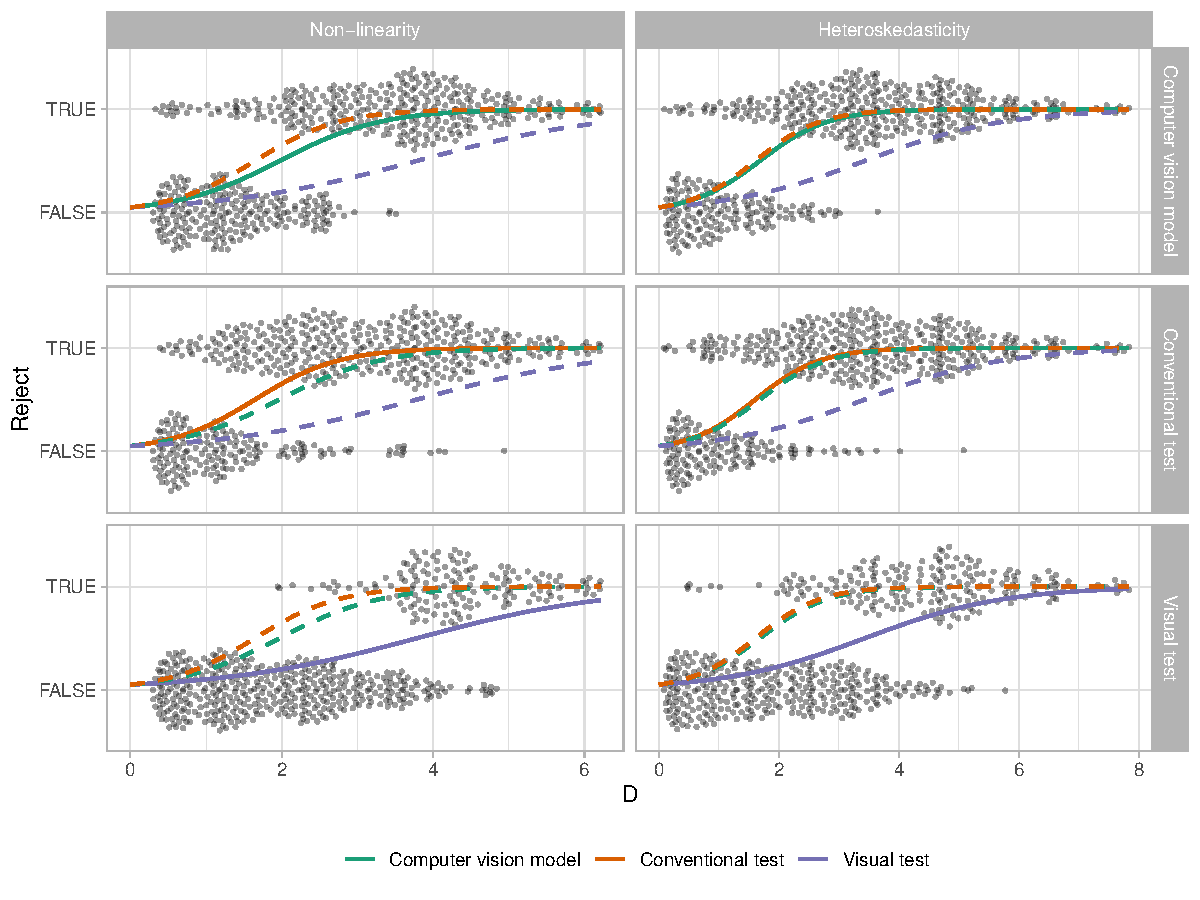
\includegraphics[width=1\linewidth]{paper_files/figure-latex/power-1} 

}

\caption{Comparison of decisions made by visual tests, conventional tests and the computer vision model. The data points are fitted with logistic regression models with no intercept but an offset equals to $\text{log}(0.05/0.95)$.}\label{fig:power}
\end{figure}

\begin{figure}[!h]

{\centering 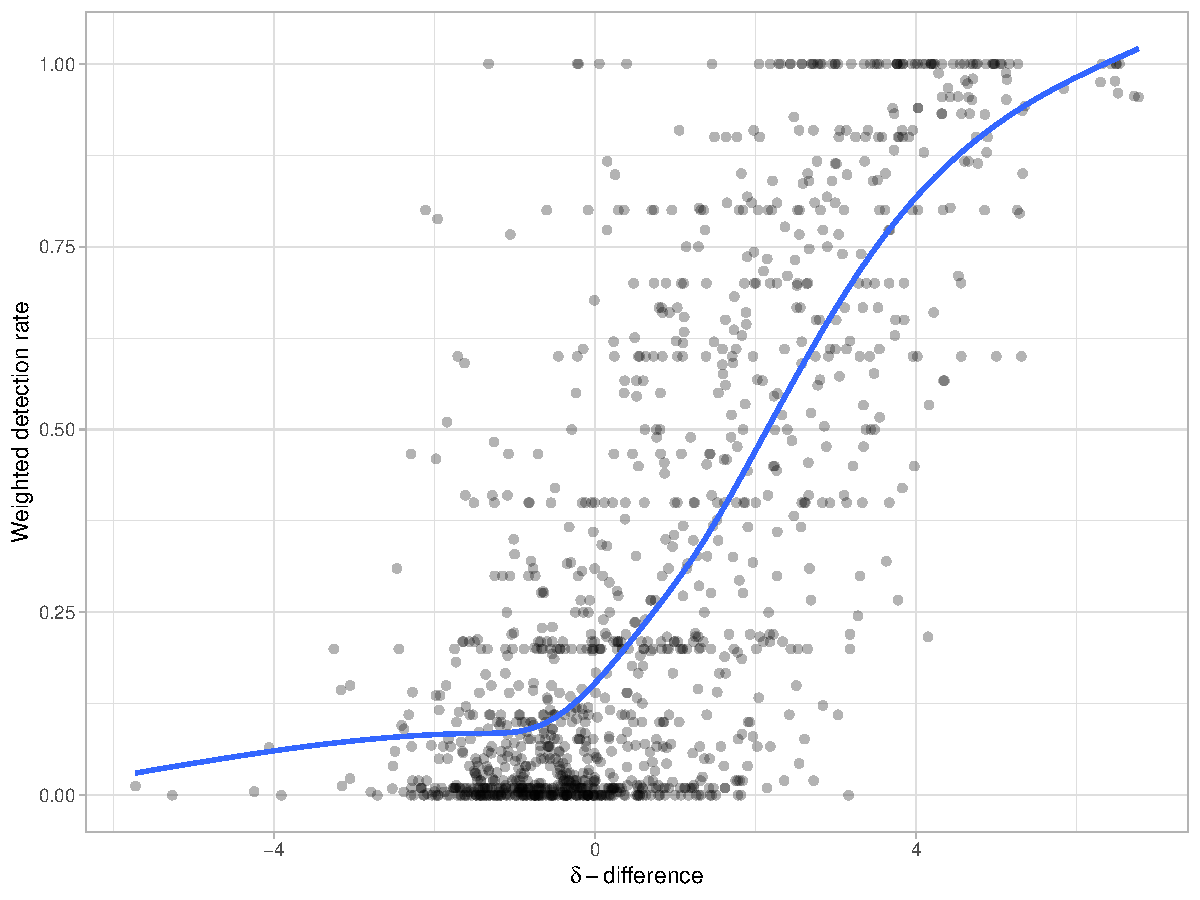
\includegraphics[width=1\linewidth]{paper_files/figure-latex/delta-1} 

}

\caption{A weighted detection rate vs $\delta$-differnence plot.}\label{fig:delta}
\end{figure}

\hypertarget{data-examples}{%
\subsection{Data examples}\label{data-examples}}

In this section, we will utilize the trained computer vision model on
three example datasets. These include the dataset associated with the
residual plot displaying a ``left-triangle'' shape, as displayed in
Figure \ref{fig:false-finding}, along with the Boston housing dataset,
and the ``dino'' datasets from the \texttt{datasaurus} R package.
Additionally, we will outline the workflow for employing this model with
the \texttt{autovi} R package.

\hypertarget{left-triangle}{%
\subsubsection{Left-triangle}\label{left-triangle}}

In Section \ref{introduction}, we presented an example residual plot
showcased in Figure \ref{fig:false-finding}, illustrating how humans
might misinterpret the ``left-triangle'' shape as indicative of
heteroskedasticity. Additionally, the Breusch-Pagan test yielded a
rejection with a \(p\)-value of 0.046, despite the residuals originating
from a correctly specified model. Figure \ref{fig:false-lineup} offers a
lineup for this fitted model, showcasing various degrees of
``left-triangle'' shape across all residual plots. This phenomenon is
evidently caused by the skewed distribution of the fitted values.
Notably, if the residual plot were evaluated through a visual test, it
would not be rejected since the actual residual plot positioned at 10
can not be distinguished from the others.

Moving forward, we will employ the trained computer vision model to
assess the residual plot with the assistance of the \texttt{autovi} R
package. This package is accessible on the GitHub repository
\texttt{TengMCing/autovi}, and users can install it by executing the
command \texttt{remotes::install\_github("TengMCing/autovi")} in R.

The results of the \texttt{list\_keras\_model()} function provide a list
of available trained computer vision models. To perform the residual
plot assessment, users need to supply a fitted linear regression model
and select a trained Keras model to initialize the checker.

\begin{Shaded}
\begin{Highlighting}[]
\NormalTok{checker }\OtherTok{\textless{}{-}} \FunctionTok{auto\_vi}\NormalTok{(}\AttributeTok{fitted\_mod =}\NormalTok{ mod, }
                   \AttributeTok{keras\_mod =} \FunctionTok{get\_keras\_model}\NormalTok{(}\StringTok{"vss\_phn\_32"}\NormalTok{))}
\end{Highlighting}
\end{Shaded}

When invoking the \texttt{check()} method to execute the assessment,
users can specify the number of null plots and bootstrapped samples
using the \texttt{null\_draws} and \texttt{boot\_draws} arguments,
respectively. The diagnostic results can be viewed by directly printing
the object. Alternatively, a summary plot of the assessment can be
generated using the \texttt{summary\_plot()} method.

\begin{Shaded}
\begin{Highlighting}[]
\NormalTok{checker}\SpecialCharTok{$}\FunctionTok{check}\NormalTok{(}\AttributeTok{null\_draws =}\NormalTok{ 200L, }\AttributeTok{boot\_draws =}\NormalTok{ 200L)}
\NormalTok{checker}\SpecialCharTok{$}\FunctionTok{summary\_plot}\NormalTok{()}
\end{Highlighting}
\end{Shaded}

Figure \ref{fig:false-check} presents the results of the assessment.
Notably, the observed visual signal strength is considerably lower than
the 95\% sample quantile of the null distribution. Moreover, the
bootstrapped distribution suggests that it is highly improbable for the
fitted model to be misspecified as the majority of bootstrapped fitted
models will not be rejected.

Thus, for this particular fitted model, both the visual test and the
computer vision model will not reject \(H_0\). However, the
Breusch-Pagan test will reject \(H_0\) because it can not effectively
utilize information from null plots.

\begin{figure}[!h]

{\centering 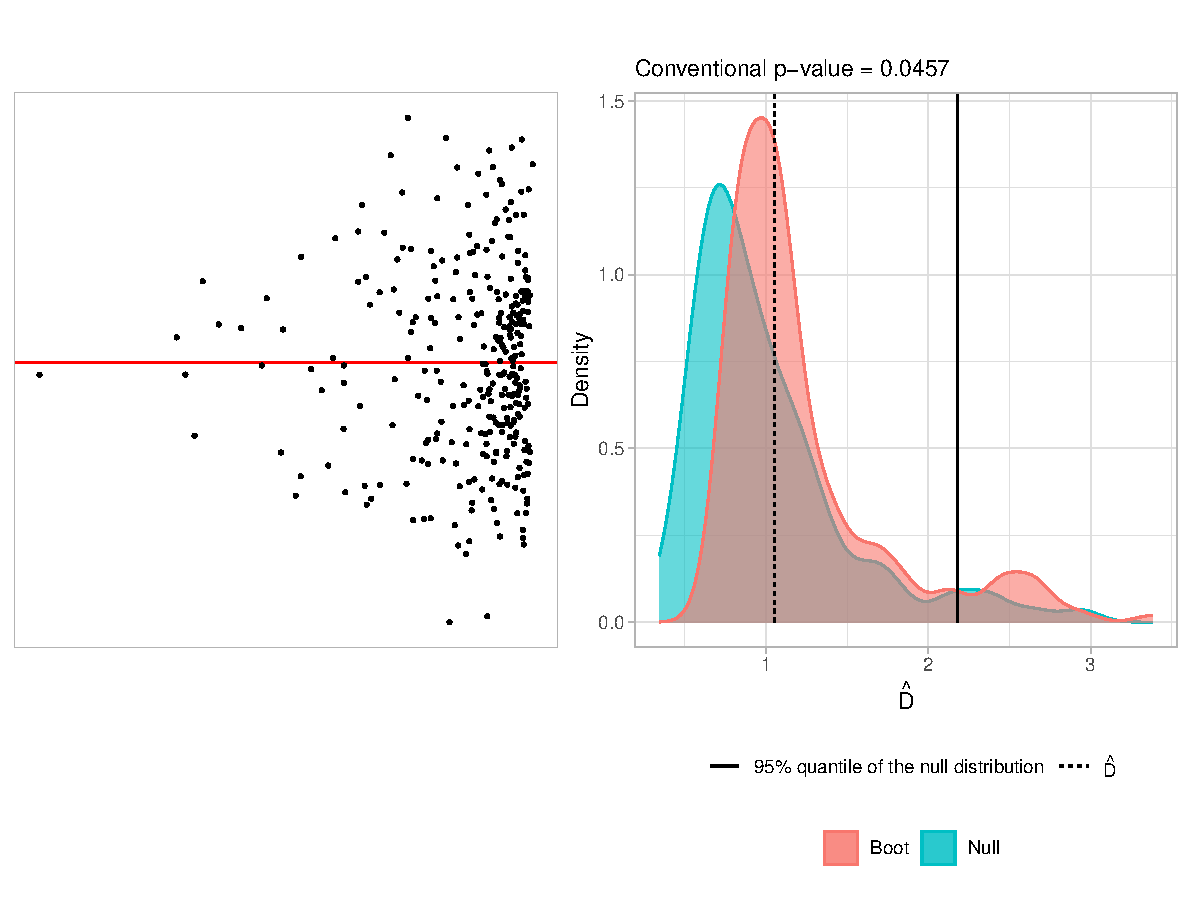
\includegraphics[width=1\linewidth]{paper_files/figure-latex/false-check-1} 

}

\caption{A summary of the residual plot assessment evaluted on 200 null plots and 200 bootstrapped plots. On the left, the residual plot exhibiting "left-triangle" shape is displayed. The blue area indicates the distribution of approximated distances for null plots, while the red area represents the distribution of approximated distances for bootstrapped plots. The fitted model will not be rejected since $\hat{D} < Q_{null}(0.95)$.}\label{fig:false-check}
\end{figure}

\begin{figure}[!h]

{\centering 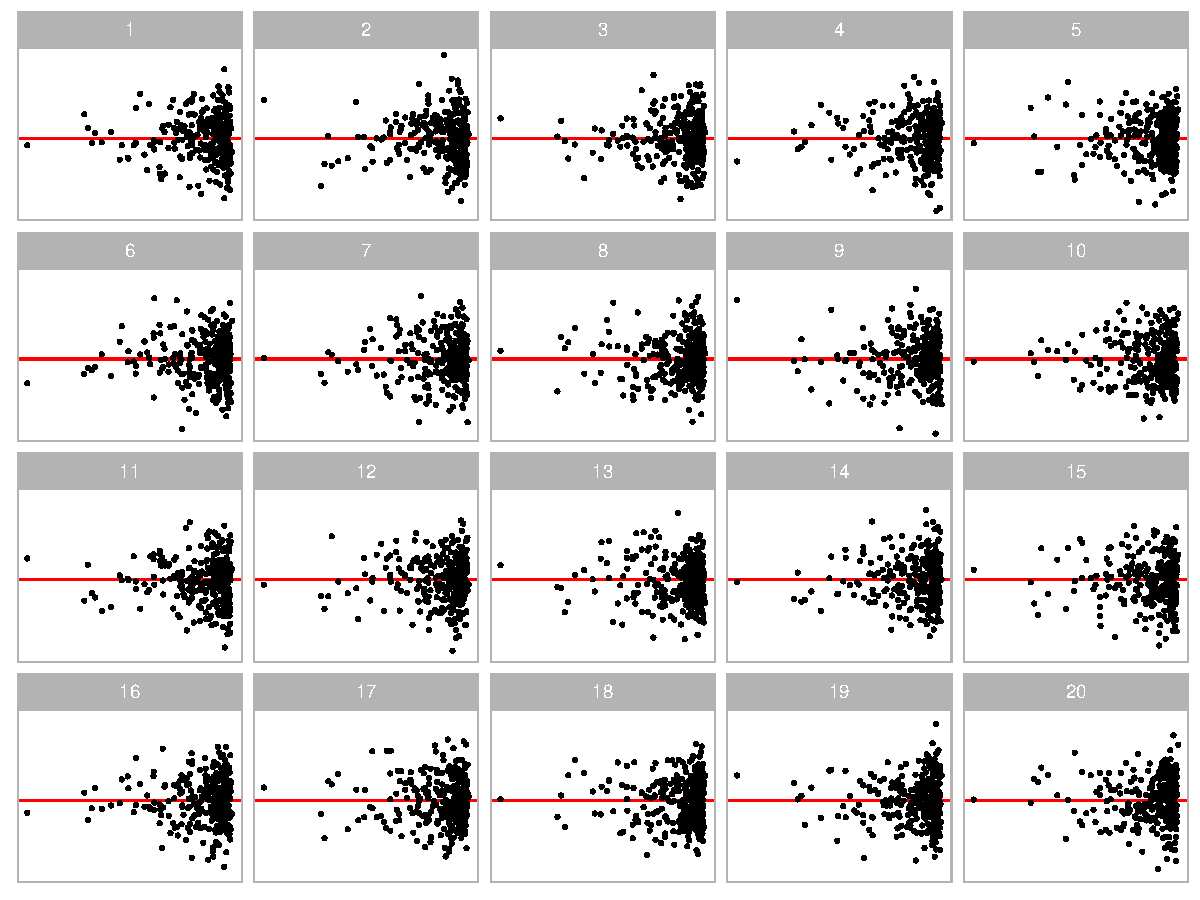
\includegraphics[width=1\linewidth]{paper_files/figure-latex/false-lineup-1} 

}

\caption{A lineup of residual plots displaying "left-triangle" visual patterns. The actual residual plot occupies position 10, yet there are no discernible visual patterns that distinguish it from the other plots.}\label{fig:false-lineup}
\end{figure}

\hypertarget{boston-housing}{%
\subsubsection{Boston housing}\label{boston-housing}}

The Boston housing dataset, originally published by
\citet{harrison1978hedonic}, offers insights into housing in the Boston,
Massachusetts area. For illustration purposes, we will utilize a reduced
version from Kaggle, comprising 489 rows and 4 columns: average number
of rooms per dwelling (RM), percentage of lower status of the population
(LSTAT), pupil-teacher ratio by town (PTRATIO), and Median value of
owner-occupied homes in \$1000's (MEDV). In our analysis, MEDV will
serve as the response variable, while the other columns will function as
predictors in a linear regression model. Our primary focus is to detect
non-linearity, because the relationships between RM and MEDV or LSTAT
and MEDV are non-linear.

Figure \ref{fig:boston-check} displays the residual plot and the
assessment conducted by the computer vision model. A clear non-linearity
pattern resembling a ``U'' shape is shown in the residual plot.
Furthermore, the RESET test yields a very small \(p\)-value. The
approximated distance \(\hat{D}\) significantly exceeds
\(Q_{null}(0.95)\), leading to rejection of \(H_0\). The bootstrapped
distribution also suggests that almost all the bootstrapped fitted
models will be rejected, indicating that the fitted model is unlikely to
be correctly specified.

Additionally, the lineup of this fitted model presented in Figure
\ref{fig:boston-lineup} underscores that the ``U'' shape is a
distinctive characteristic of the actual residual plot, absent in any of
the null plots. Consequently, if a visual test is conducted, \(H_0\)
will also be rejected.

\begin{figure}[!h]

{\centering 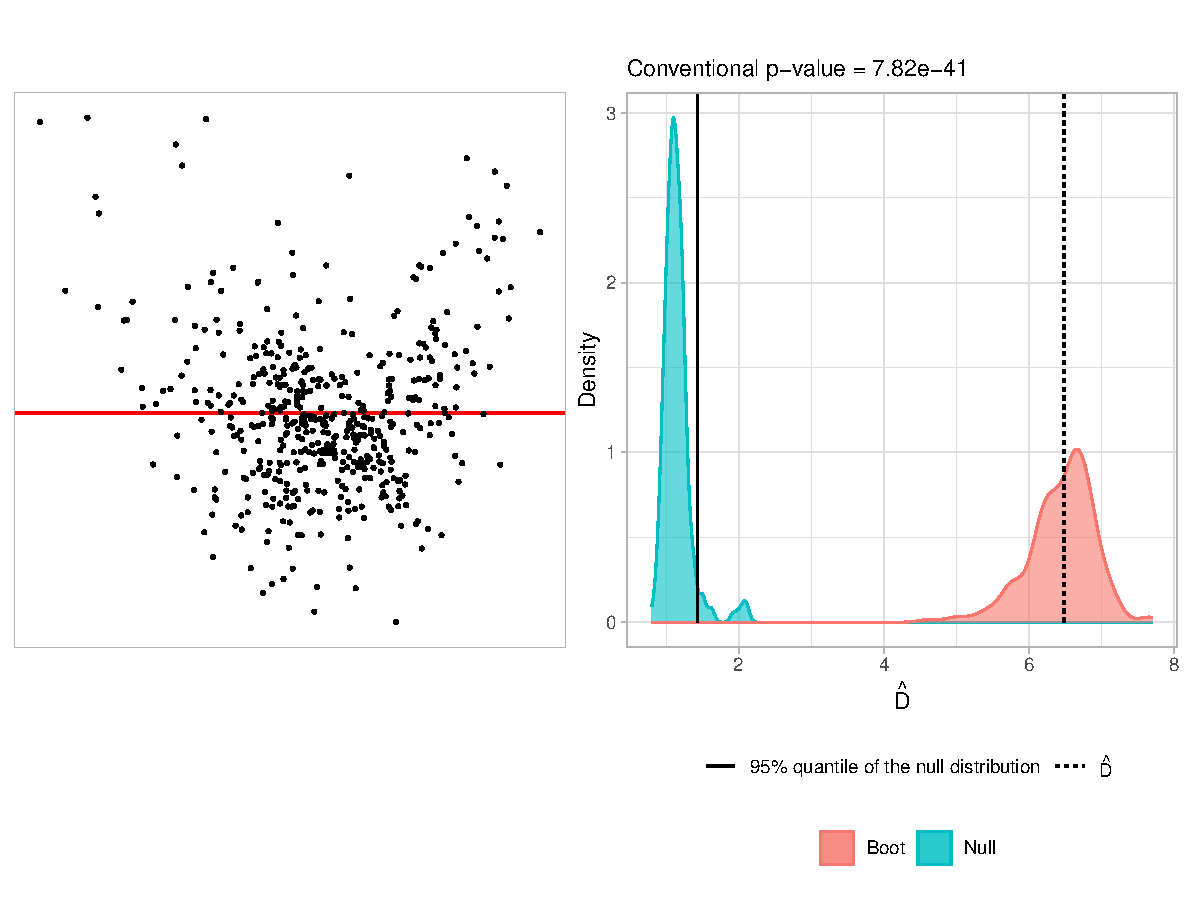
\includegraphics[width=1\linewidth]{paper_files/figure-latex/boston-check-1} 

}

\caption{A summary of the residual plot assessment evaluted on 200 null plots and 200 bootstrapped plots. On the left, the residual plot of the Boston housing fitted model is displayed. The blue area indicates the distribution of approximated distances for null plots, while the red area represents the distribution of approximated distances for bootstrapped plots. The fitted model will be rejected since $\hat{D} >= Q_{null}(0.95)$.}\label{fig:boston-check}
\end{figure}

\begin{figure}[!h]

{\centering 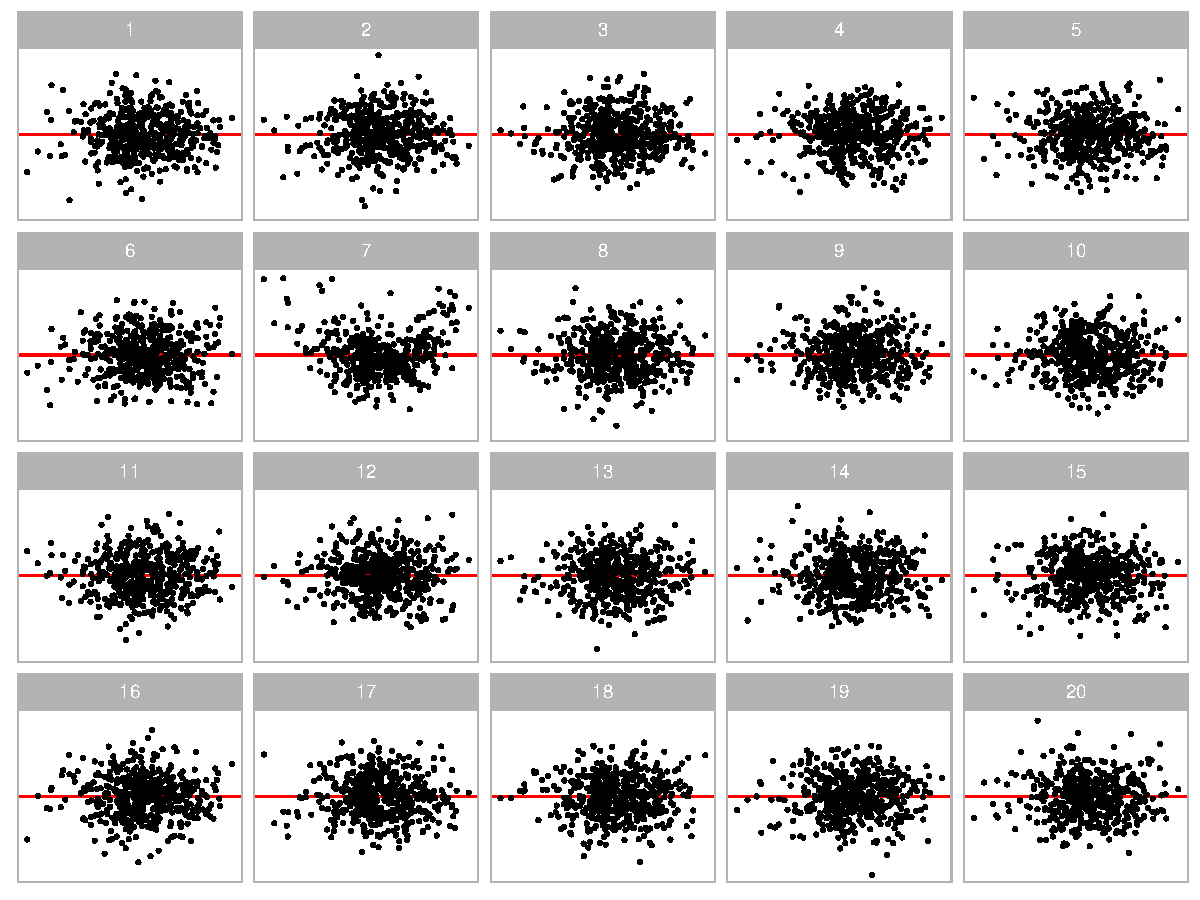
\includegraphics[width=1\linewidth]{paper_files/figure-latex/boston-lineup-1} 

}

\caption{A lineup of residual plots for the Boston housing fitted model. The actual residual plot is at position 7. It can be easily identified as the most different plot.}\label{fig:boston-lineup}
\end{figure}

\hypertarget{datasaurus}{%
\subsubsection{Datasaurus}\label{datasaurus}}

The computer vision model possesses the capability to detect not only
typical issues like non-linearity, heteroskedasticity, and non-normality
but also artifact visual patterns resembling real-world objects, as long
as they do not appear in null plots. These visual patterns can be
challenging to categorize in terms of model violations. Therefore, we
will employ the RESET test, the Breusch-Pagan test, and the Shapiro-Wilk
test \citep{shapiro1965analysis} for comparison.

The ``dino'' dataset within the \texttt{datasaurus} R package
exemplifies this scenario. With only two columns, x and y, fitting a
regression model to this data yields a residual plot resembling a
``dinosaur,'' as displayed in Figure \ref{fig:dino-check}.
Unsurprisingly, this distinct residual plot stands out in a lineup, as
shown in Figure \ref{fig:dino-lineup}. A visual test conducted by humans
would undoubtedly reject \(H_0\).

According to the residual plot assessment by the computer vision model,
\(\hat{D}\) exceeds \(Q_{null}(0.95)\), warranting a rejection of
\(H_0\). Additionally, most of the bootstrapped fitted models will be
rejected, indicating an misspecified model. However, both the RESET test
and the Breusch-Pagan test yield \(p\)-values greater than 0.3, leading
to a non-rejection of \(H_0\). Only the Shapiro-Wilk test rejects the
normality assumption with a small \(p\)-value.

In practice, without accessing the residual plot, it would be
challenging to identify the artificial pattern of the residuals.
Moreover, conducting a normality test for a fitted regression model is
not always standard practice among analysts. Even when performed,
violating the normality assumption is sometimes deemed acceptable,
especially considering the application of quasi-maximum likelihood
estimation in linear regression. This example underscores the importance
of evaluating residual plots and highlights how the proposed computer
vision model can facilitate this process.

\begin{figure}[!h]

{\centering 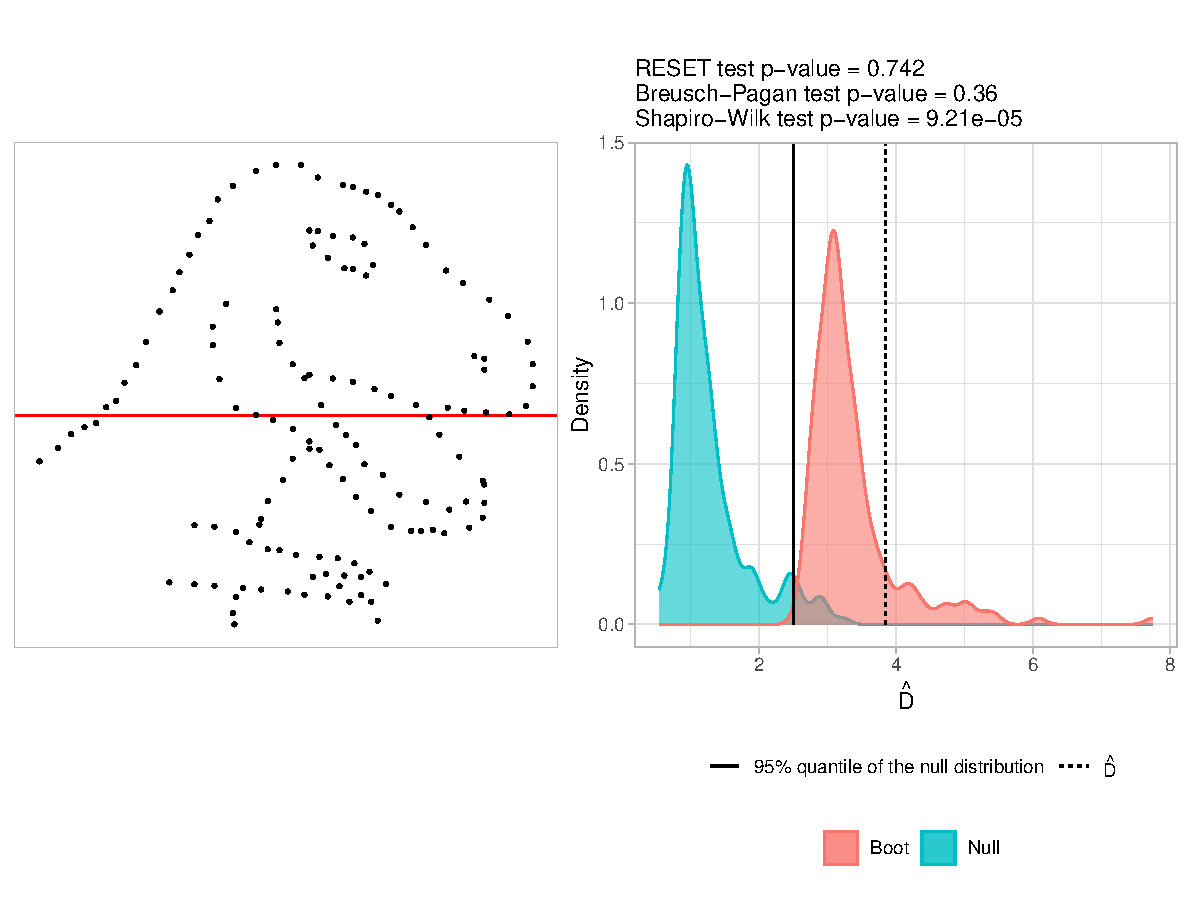
\includegraphics[width=1\linewidth]{paper_files/figure-latex/dino-check-1} 

}

\caption{A summary of the residual plot assessment evaluted on 200 null plots and 200 bootstrapped plots. On the left, the residual plot exhitbiting a "dinosaur" shape is displayed. The blue area indicates the distribution of approximated distances for null plots, while the red area represents the distribution of approximated distances for bootstrapped plots. The fitted model will be rejected since $\hat{D} >= Q_{null}(0.95)$.}\label{fig:dino-check}
\end{figure}

\begin{figure}[!h]

{\centering 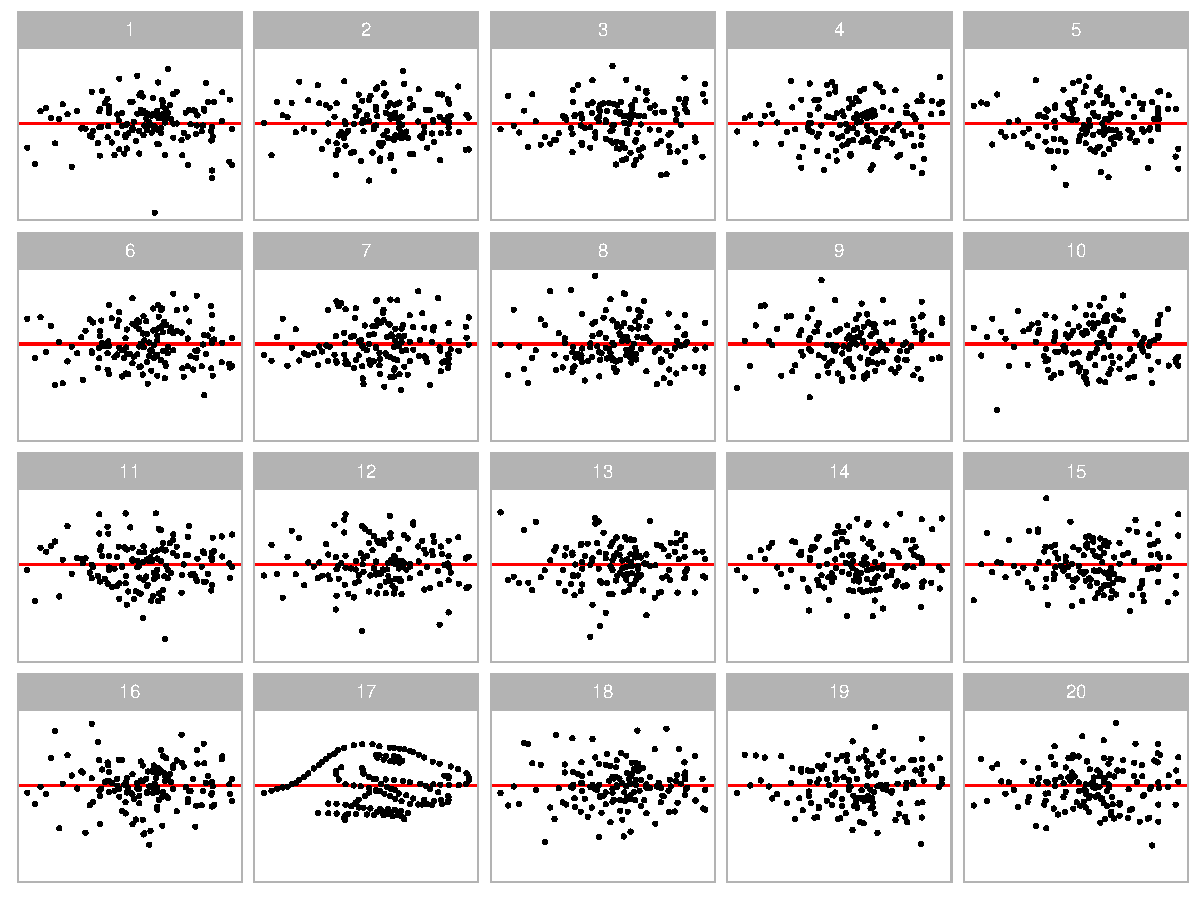
\includegraphics[width=1\linewidth]{paper_files/figure-latex/dino-lineup-1} 

}

\caption{A lineup of residual plots for the fitted model on the "dinosaur" dataset. The actual residual plot is at position 17. It can be easily identified as the most different plot as the visual pattern is extremly artificial.}\label{fig:dino-lineup}
\end{figure}

\hypertarget{conclusion}{%
\section{Conclusion}\label{conclusion}}

\begin{itemize}
\tightlist
\item
  Brief discussion
\item
  Summary of findings
\item
  Contributions to the field
\end{itemize}

In this study, we have introduced a distance metric based on
Kullback-Leibler divergence to quantify the disparity between the
residual distribution of a fitted linear regression model and the
reference residual distribution assumed under correct model
specification. This distance metric effectively captures the magnitude
of model violations in misspecified models. We propose a computer vision
model to approximate this distance, utilizing the residual plot of the
fitted model as input. The resulting approximated distance serves as the
foundation for constructing a single Model Violation Index (MVI),
facilitating the quantification of various model violations.

Moreover, the approximated distance enables the development of a formal
statistical testing procedure by evaluating a large number of null plots
generated from the fitted model. Additionally, employing bootstrapping
techniques and refitting the regression model allows us to ascertain how
frequently the fitted model is considered misspecified if data were
repeatedly obtained from the same data generating process.

The trained computer vision model demonstrates strong performance on
both the training and test sets, although it exhibits slightly lower
performance on residual plots with non-linearity visual patterns
compared to other types of violations. The statistical tests relying on
the approximated distance predicted by the computer vision model exhibit
lower sensitivity compared to conventional tests but higher sensitivity
compared to visual tests conducted by humans. While the approximated
distance generally mirrors the strength of the visual signal perceived
by humans, there remains scope for further improvement in its
performance.

Several examples are provided to showcase the effectiveness of the
proposed method across different scenarios, emphasizing the similarity
between visual tests and distance-based tests. Overall, both visual
tests and distance-based tests can be viewed as combined tests, aiming
to assess the correctness of all model assumptions collectively. In
contrast, individual residual diagnostic tests such as the RESET test
and the Breusch-Pagan test only evaluate specific model assumptions.

In practice, selecting an appropriate set of statistical tests for
regression diagnostics can be challenging, particularly given the
necessity of adjusting the significance level for each test.

Our method holds significant value as it helps alleviate a portion of
analysts' workload associated with assessing residual plots. While we
recommend analysts to continue reading residual plots whenever feasible,
as they offer invaluable insights, our approach serves as a valuable
tool for automating the diagnostic process or for supplementary purposes
when needed.

\begin{itemize}
\tightlist
\item
  Future directions
\end{itemize}

\hypertarget{acknowledgements}{%
\section*{Acknowledgements}\label{acknowledgements}}
\addcontentsline{toc}{section}{Acknowledgements}

\begin{itemize}
\tightlist
\item
  Packages used
\item
  Website link
\end{itemize}

\bibliographystyle{tfcad}
\bibliography{ref.bib}





\end{document}
